\pagestyle{fancy} \rhead{\bfseries OCR A-Level Computer Science}
\chead{\mdseries \thepage}
\lhead{\bfseries Jonathan Kasongo \mdseries — May 2025/26}
\lfoot{\sffamily Candidate number: N/A}
\rfoot{\sffamily Centre number: N/A}

\chapter{Development}
\label{chap:development}

% Provided evidence of each stage of the iterative
% development process for a coded solution
% relating this to the break down of the problem
% from the analysis stage and explaining what they
% did and justifying why.

% Well structured and modular, code annotated, DRY

% Validation evidence

\section{Development overview and sub-tasks}

We apply the principle of decomposition to our development
plan by splitting up the development of the system into
a number of smaller sub-tasks. Each sub-task relates to it's
relevant circled number in our problem breakdown (see section
\ref{sec:breakdown}).\\ \vspace{0.2cm}

In doing this we \textbf{clearly} relate each iteration
to a part of the problem breakdown.\\ \vspace{0.2cm}

\begin{longtblr}[
  caption={Development sub-tasks.}
]{
  colspec={cX}, row{1}={lightestgray}
}
  Number & Sub-task \\
  \circled{1} & Design home page \\
  \circled{1.1} & Design help page \\
  \circled{1.2} & Design login page \\
  \circled{1.3} & Document the backend code throughout\\
  \circled{2} & Allow users to create their account\\
  \circled{3} & Implement login system with password resets \\
  \circled{6} & Implement a settings page \\
  \circled{7} & Implement a create call page \\
  \circled{8} & Implement a join call page \\
  \circled{A} & Deploy website \\
  \circled{B} & Complete video-conferencing system backend \\
\end{longtblr}
\vspace{0.2cm}

Finally note that all the code for this project is open source
and freely available for you to view on github:
\url{https://github.com/zzzNathan/Video-Conferencer}. \\ \vspace{0.2cm}

\textit{We may shorten code snippets using ellipsis though the
entire code at such point in development is available by finding the
correct commit on Github. This commit number as well a link are both
provided at the end of each iteration.}

\section{Iteration 1}

% explaining what they did and justifying why

During this iteration I wanted to finish up designs for a few
of the pages that will appear on our website. This should
clear up sub-task \circled{1} and \circled{1.2}.

\subsubsection{Home page}

\begin{figure}[H]
\centering

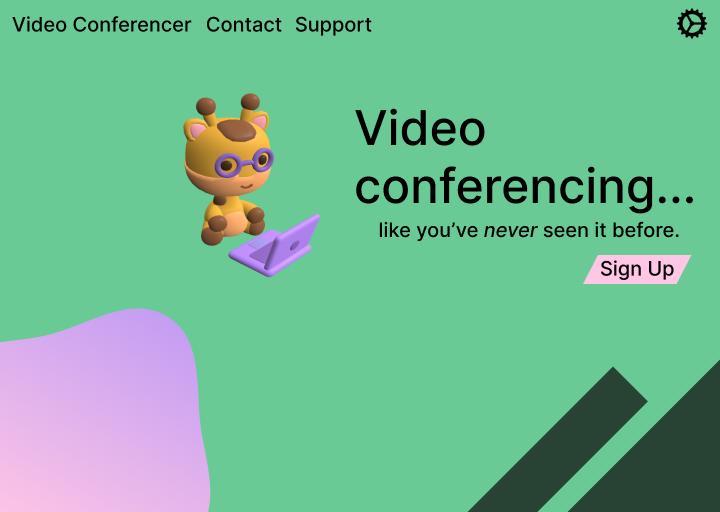
\includegraphics[scale=0.2]{Images/HomeUI_2.png}

\caption{2nd Mock up of the home page.}
\label{fig:ui2}
\end{figure}

\begin{figure}[H]
\centering

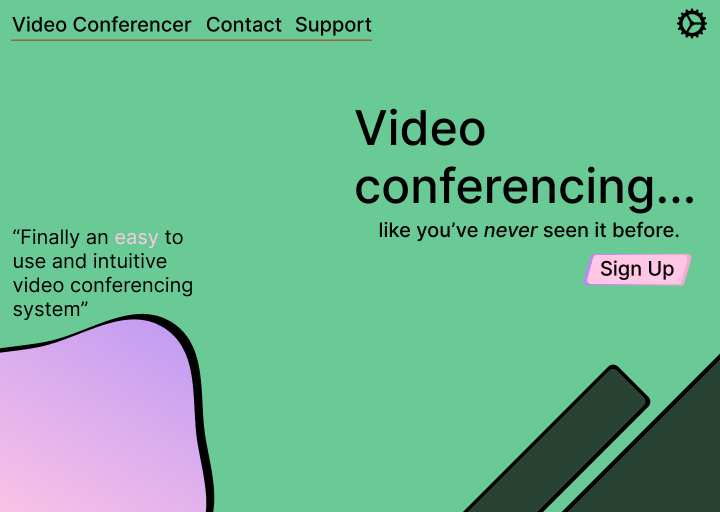
\includegraphics[scale=0.2]{Images/HomeUI_3.png}

\caption{3rd Mock up of the home page.}
\label{fig:ui3}
\end{figure}

\textit{Description:}
I started by cleaning up the mock design for our home page.
The first mock up was a very basic outline for how I wanted to
style the page, so in the next couple iterations I polished
the design and added more designs to fill the web page. These
additions made the home page feel more complete and less
bare-bones, consequently making the webpage feel more
professional for the user. \\ \vspace{0.2cm}

\textit{Explanation and justification:}
I created mock ups of the home page and all other web pages
before actually coding them up. Designing mock ups helped
to give me a sense of direction in the process of creating a
webpage design in HTML and CSS. If I were to try to create
the design on the fly whilst writing code I would have no
reference to use and my design would end up being lackluster
and poorly thought out. By purely focusing on the page layout
and design first, I can create a page that I am happy with in
Figma and then focus on converting this design into HTML and
CSS code using my mock ups as a reference as to what the end
product should look like. Indeed by starting with designing
mock ups, it gives me something to aim for when writing up
the code to produce our home page. Then by iteratively
improving upon the design mock ups I created I enhance
the look of the final home page design, in turn creating
a superior user experience.
\\ \vspace{0.2cm}

\textit{Description:}
I transfer my designs into HTML and CSS. However after some
reseach I come to the conclusion that I'd prefer to write
sass and compile this into CSS instead, because of it's
superior syntax. \\ \vspace{0.2cm}

\textit{Explanation and justification:}
The next step was to transfer this design into HTML and CSS.
Since my designs made use of a collection of frequently used
colours I concluded that it would be useful to be able to use
these colours as defined variables instead of having to write
out their hex colour codes each time
(see section \ref{sec:ui}). However the native CSS syntax
looks something like this. (Taken from \url{https://www.w3schools.com/css/css3_variables.asp})

\begin{minted}[linenos, bgcolor=lightestgray]{css}
:root {
  --blue: #1e90ff;
  --white: #ffffff;
}
\end{minted}

I personally found this syntax particularly disgusting,
after doing some research I came across this stack overflow
answer \url{https://stackoverflow.com/a/1877358}. After digging
into exactly what "sass" and "less" were I decided to use sass
as an extension of my CSS because I liked the look of it's
syntax better. Sass (\textbf{S}yntactically \textbf{A}wesome
\textbf{S}tylesheet) is a CSS extension language that
provides a new syntax for writing CSS as well as a number of
features that prevent repetition in the code like variables,
functions and more. The sass code is saved in a \texttt{.sass}
file then one can compile the sass code into CSS by using the
command \texttt{sass <sass file name> <output css file name>}.
\\ \vspace{0.2cm}

After blocking in the basic elements of our webpage the HTML
and sass code looked like this.

\subsubsection{Prototype 1}

\underline{main.html}

\begin{minted}[linenos, bgcolor=lightestgray]{html}
<!DOCTYPE html>
<html>

<head>
  <meta charset="UTF-8">
  <meta name="viewport" content="width=device-width, initial-scale=1.0">
  <link href='https://fonts.googleapis.com/css?family=Inter' rel='stylesheet'>
  <link rel="stylesheet" href="styles.css">
  <title>Video-Conferencer</title>
</head>

<body>
  <div class="Headlines">

    <div class="Main_Headline">
      Video conferencing...
    </div>

    <div class="Sub_Headline">
      like you've never seen before.
    </div>

  </div>
</body>

</html>
\end{minted}

\underline{styles.sass}

\begin{minted}[linenos, bgcolor=lightestgray]{sass}
// Colour definitions
$Col_Main:       #69ca95
$Col_Secondary:  #284333
$Col_Tertiary:   #9a6442
$Col_Accent:     #ffc6e5
$Col_AccentDark: #c49df2

// Setting font and background colour
body
  background-color: $Col_Main
  font-family:      'Inter', sans-serif

// Styling for the main headline
.Main_Headline
  width:       701px
  height:      238px
  font-size:   96px
  ...

// Styling for the sub headline
.Sub_Headline
  width:       603px
  height:      101px
  font-weight: 500
  ...
\end{minted}

This code produced our 1st prototype.

\begin{figure}[H]
\centering


\includegraphics[scale=0.2]{Images/Proto_home1.png}

\caption{Home page prototype 1}
\end{figure}

{\color{gray} \hrulefill} \\ \vspace{0.2cm}

{\sffamily Client Feedback:}
\begin{itemize}
  \item The headline and sub-headline are too far apart.
  \item The main headline takes up too much space on the page.
  \item The "never" isn't italicised.
\end{itemize}

{\color{gray} \hrulefill}

\subsubsection{Prototype 2}

\textit{Description:}
I pivot to using vector graphics in order to position the
elements on our webpage. \\ \vspace{0.2cm}

\textit{Explanation and justification:}
After writing the code for the first prototype I soon realised
that actually writing the text for the main headlines and
manually positioning it would be a very tedious task. So I
decided to instead export the headline as well as the graphic
designs as \texttt{.svg} files from Figma. This means I
wouldn't have to worry about carefully positioning and spacing
the headlines individually and I could instead just position
them as 1 vector image. The \texttt{.svg} image format was
chosen because vector images never lose their resolution even
when scaled, you will still be able to see clean and crisp
images no matter how much you zoom in, something which isn't
achievable with the \texttt{.jpg} or the \texttt{.png} formats.
In the rare case that \texttt{.svg} files are not supported
for the user's browser \footnote{Vector images are supported
by all browser except Internet Explorer 8 and below, and
Android 2.3 browser and below.} we also provide fallback
\texttt{.png} image files for these users. This ensures that
users will be able to see the page's content no matter their
choice of browser, hence improving the robustness of our
system.\\ \vspace{0.2cm}

Our code now looks like this.

\underline{main.html}
\begin{minted}[linenos, bgcolor=lightestgray]{html}
...

<body>

  <div id="Headline_container">
    <object id="Headline" data="Images/Headline_text.svg" type="image/svg+xml">
      <img src="Images/Headline_text.png">
    </object>

    <object id="Sign_up" data="Images/Sign_up.svg" type="image/svg+xml">
      <img src="Images/Sign_up.png">
    </object>
  </div>

  <div id="Bot_left_graphic_container">
    <object id="Bot_left_graphic" data="Images/Bot_left_graphic.svg" type="image/svg+xml">
      <img src="Images/Bot_left_graphic.png">
    </object>
  </div>

  <div id="Bot_right_graphic_container">
    <object id="Bot_right_graphic" data="Images/Bot_right_graphic.svg" type="image/svg+xml">
      <img src="Images/Bot_right_graphic.png">
    </object>
  </div>

</body>

</html>
\end{minted}

\underline{styles.sass}
\begin{minted}[linenos, bgcolor=lightestgray]{sass}
...

// Setting font and background colour
body
  height:           100vh
  margin:           0
  background-color: $Col_Main
  ...

// Positioning the headline svg
#Headline_container
  position: relative
  top:      10%
  left:     45%

// Positioning the signup svg
#Sign_up
  position: absolute
  top:      75%
  left:     35%

// Positioning the bottom left graphic svg
#Bot_left_graphic_container
  position: relative
  top:      0%

// Positioning the bottom right graphic svg
#Bot_right_graphic_container
  position: relative
  left:     50%
  bottom:   75%
\end{minted}

This code produced our 2nd prototype.

\begin{figure}[H]
\centering

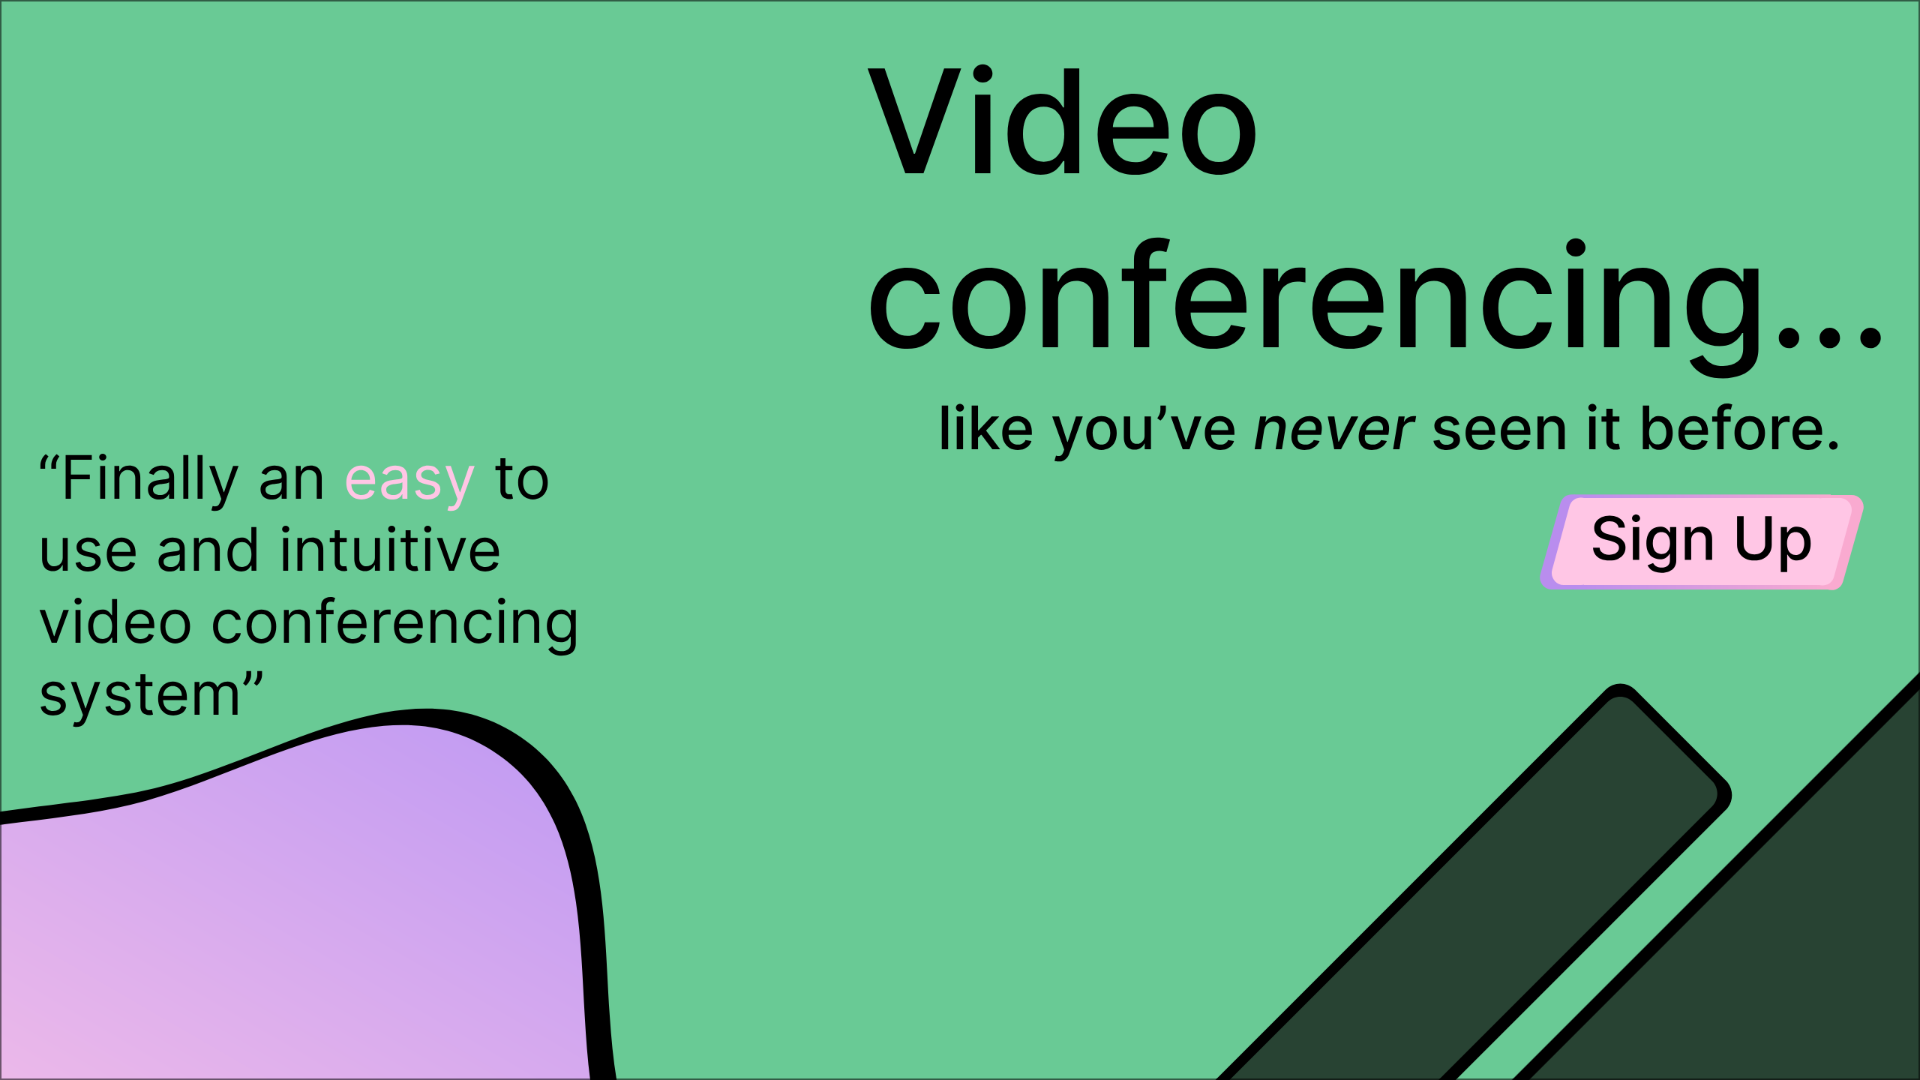
\includegraphics[scale=0.2]{Images/Proto_home2.png}

\caption{Home page prototype 2}
\end{figure}

{\color{gray} \hrulefill} \vspace{0.2cm}

{\sffamily Client feedback:}

\begin{itemize}
  \item We are still lacking a navigation bar at the top.
  \item All the elements feel as though they take up too much space on the page.
\end{itemize}

{\color{gray} \hrulefill}

\subsubsection{Prototype 3}

\textit{Description:}
I redesign the entire look and aesthetic of our system.
\\ \vspace{0.2cm}

\textit{Explanation and justification:}
After reviewing the design holistically, I felt that I could
have done a better job designing the page to contribute to
creating a professional looking system, so I re-did my
designs in Figma. The graphic designs on our previous
prototype designs were nice but they felt "too much",
so I decided I should tone back the designs and focus on
simplicity. Indeed our target user base is comprised of
elderly ones who might not appreciate such a bright and
vibrant design, the design would have not only been
overwhelming for the average user but also would have made
our system seem unprofessional and childish. This is seen
in the complete lack of cohesion between the various graphics
on that page. The dark green triangle graphic creates an
unwanted contrast between it and the rest of the page to the
point that it becomes the centre of attention and one of the
first things that will catch the user's eye.
Furthermore the choice for the background colour
was too bright and vibrant and didn't allow other elements
to stand out as much as they should.\\ \vspace{0.2cm}

In designing the revised
prototype I took inspiration from the design of the
Zen browser home-page \url{https://zen-browser.app/}. They
simply have a navigation bar, a main and sub headline, a call
to action button and some testimonials along the bottom. Here
is the newest design. (Of course after making such significant
changes I contacted my client and asked for permission to
change to this new design and he agreed). \\

\begin{figure}[H]
\centering

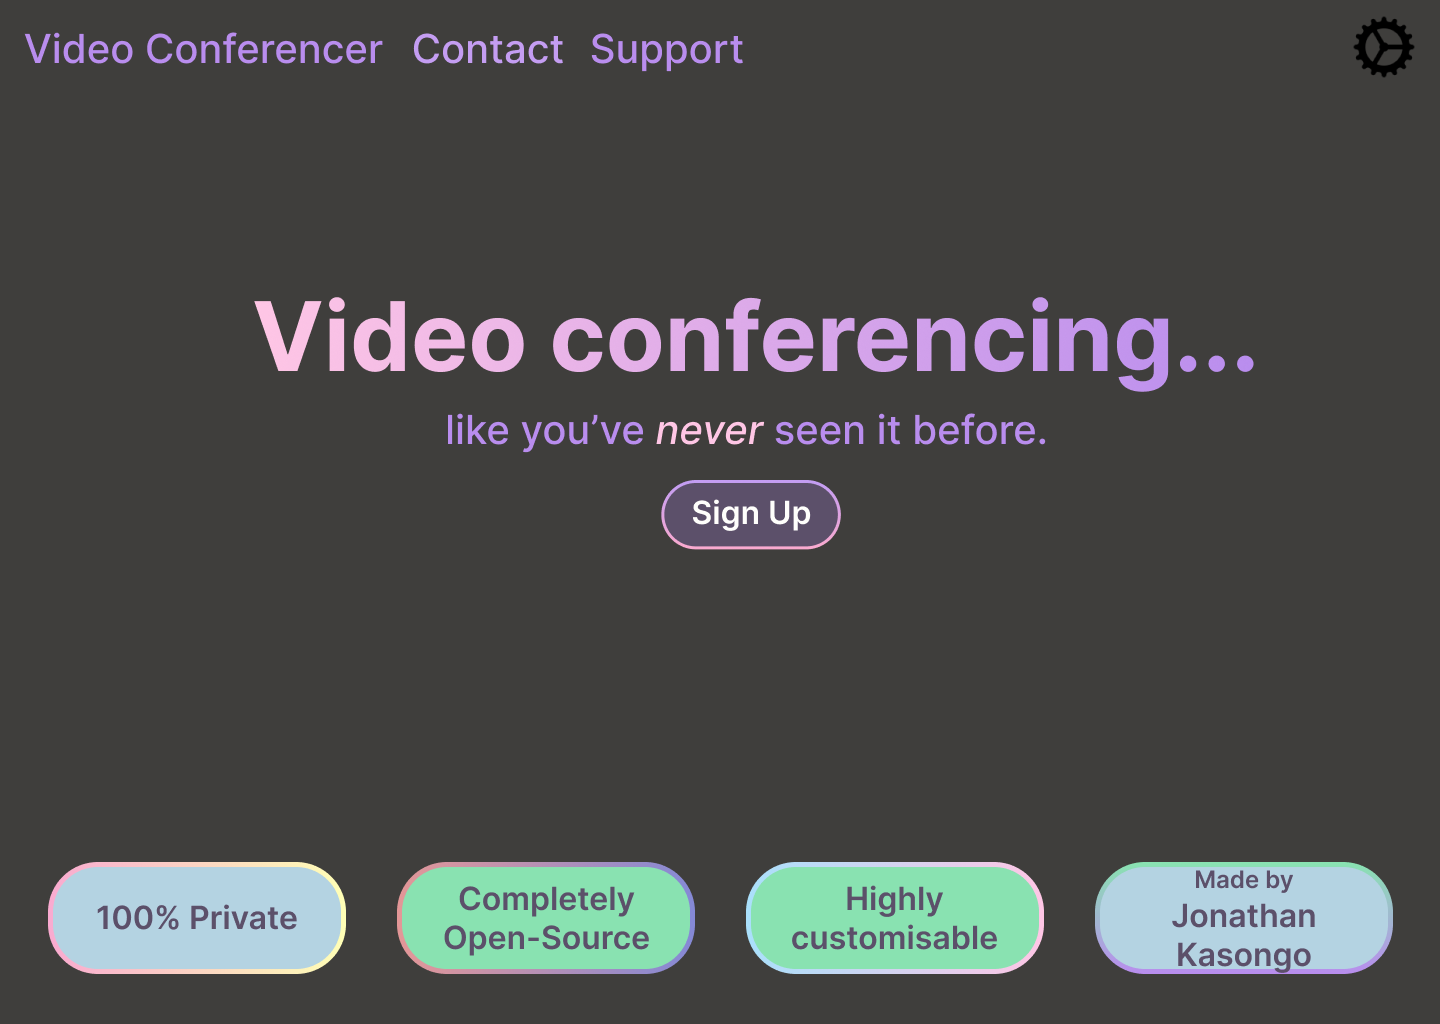
\includegraphics[scale=0.2]{Images/HomeUI_4.png}

\caption{4th Mock up of the home page.}
\end{figure}

Now in relation to the point \textit{"the elements feel as
though they take up too much space on the page"} I found that
an appropriate solution was to simply scale every element on
our page to 75\%. This then made the page look closer to the
one design in Figma. Whilst writing the HTML and sass code I
made some minor design changes based on what looked the most
appealing. The bottom bar was dropped from the final design
because it felt tacky compared to rest of the website. I
instead replaced it with the quote that sat on the bottom
left of our original design (look at prototype 2). Finally I
gave the settings icon the same purple colour as the rest of
the navigation bar. Here is the code of the 3rd prototype. \\
\vspace{0.2cm}

\underline{main.html}

\begin{minted}[linenos, bgcolor=lightestgray]{html}
  ...
  <link rel="stylesheet" href=
    "https://maxcdn.bootstrapcdn.com/bootstrap/3.3.7/css/bootstrap.min.css">
  ...
<body>

  <ul id="Navbar">

    <li id="Logo_container">
      <object id="Logo" data="Images/Logo.svg" type="image/svg+xml">
        <img src="Images/Logo.png">
      </object>
    </li>

    ...

    <li id="Settings">
      <i class="glyphicon glyphicon-cog"></i>
    </li>
  </ul>

  <div id="Main">
    <object id="Headline" data="Images/Headline.svg" type="image/svg+xml">
      <img src="Images/Headline.png">
    </object>

    <object id="Sign_up" data="Images/Sign_up.svg" type="image/svg+xml">
      <img src="Images/Sign_up.png">
    </object>
  </div>

  <object id="Quote" data="Images/Quote.svg" type="image/svg+xml">
    <img src="Images/Quote.png">
  </object>

</body>

</html>
\end{minted}

\underline{styles.sass}

\begin{minted}[linenos, bgcolor=lightestgray]{sass}
// Colour definitions
...

// Setting font and background colour
body
  height:           100vh
  margin:           0
  background-color: $Col_Main
  ...

// Positioning the headline
#Headline
  display:      block
  margin-left:  auto
  margin-right: auto
  ...

// Scaling the sign up button
#Sign_up
  margin-top: -3vh
  scale:       75%

#Navbar
  list-style-type: none
  margin:          0
  padding:         0
  ...

// Styling the navbar elements
#Settings
  float: right
  scale: 300%
  color: $Col_Secondary
  ...

#Contact_container
  margin-right: 0%
  scale:        75%
  padding:      2vh

#Logo_container
  margin-left:  -3%
  margin-right: -5%
  scale:        75%
  ...

#Support_container
  margin-left:  -3%
  margin-right: 45%
  scale:        75%
  ...

// Positioning the call to action button
#Main
  display:         flex
  align-items:     center
  justify-content: center
  flex-direction:  column

// Positioning the quote
#Quote
  position: relative
  left:     0%
  top:      20%
  ...
\end{minted}

This code produced our 3rd prototype.

\begin{figure}[H]
\centering

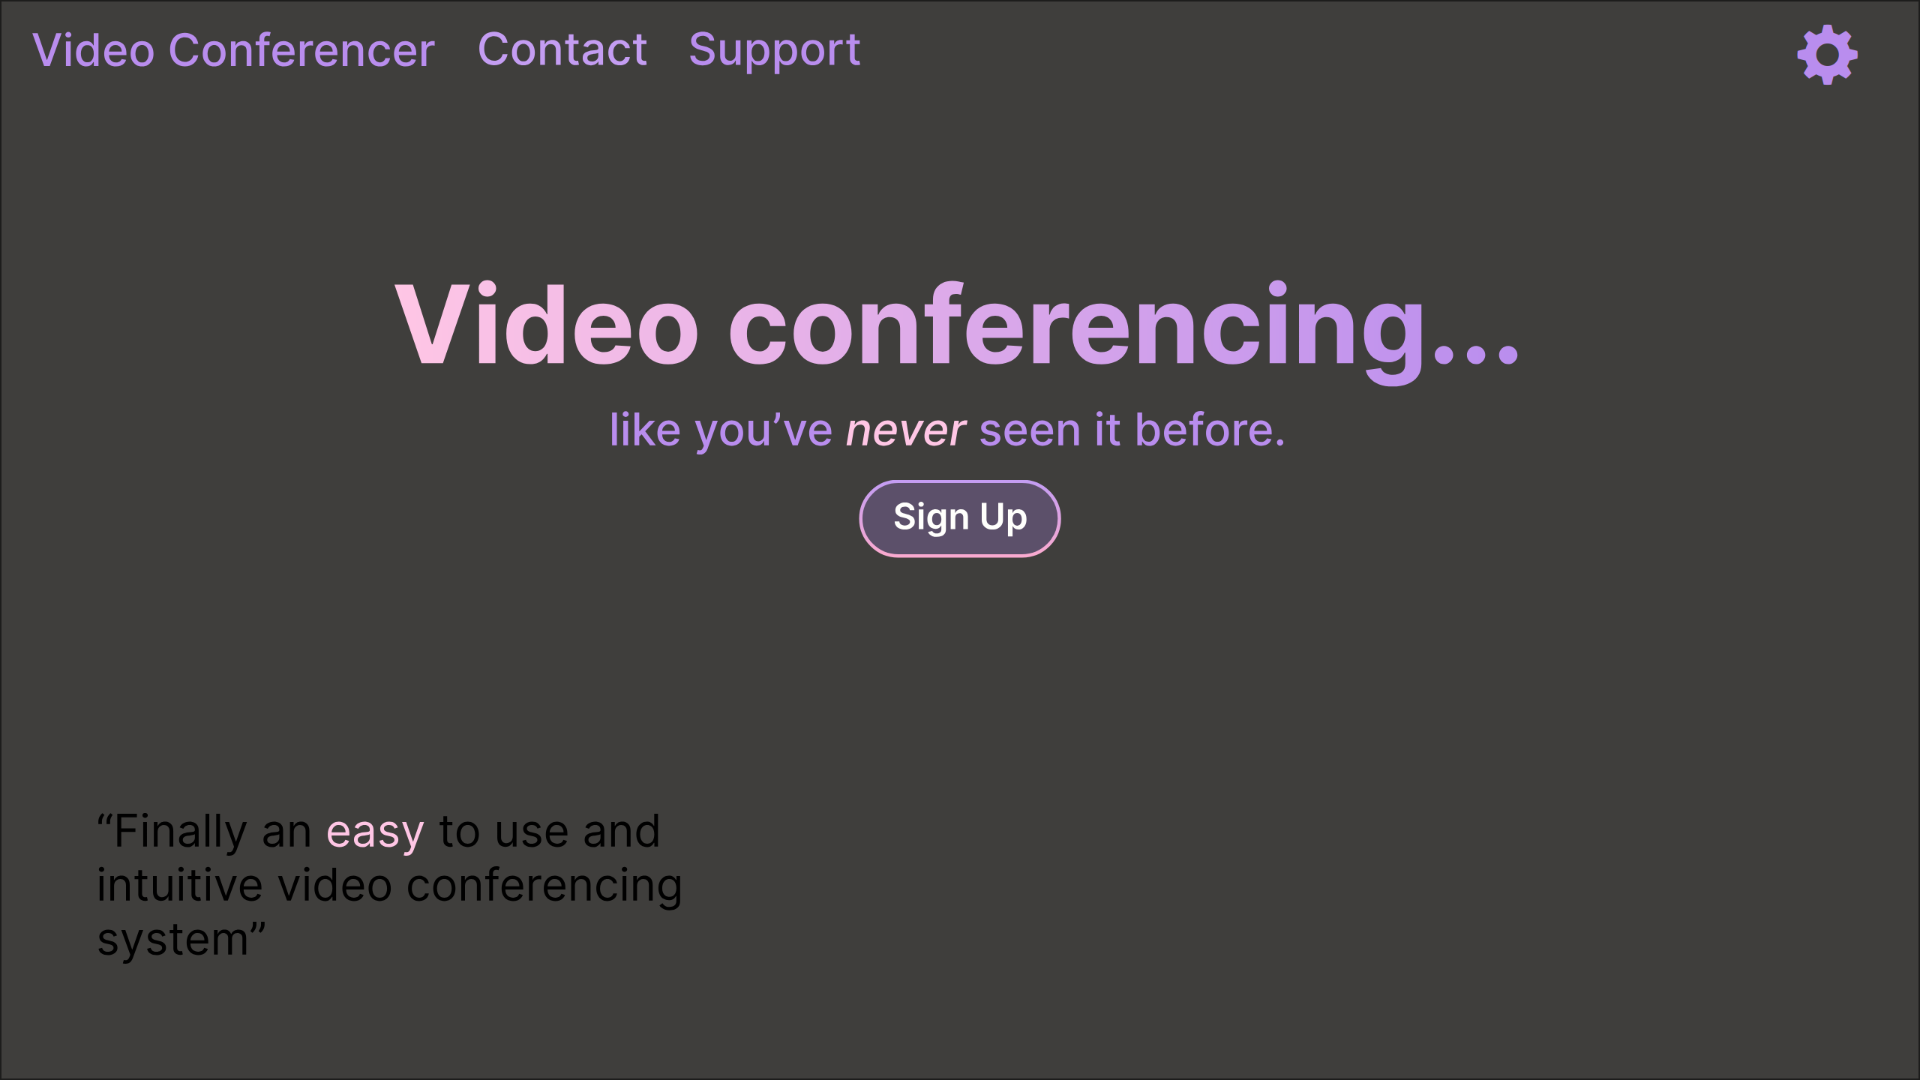
\includegraphics[scale=0.2]{Images/Proto_home3.png}

\caption{Home page prototype 3}
\end{figure}

{\color{gray} \hrulefill} \vspace{0.2cm}

{\sffamily Client feedback:}

\begin{itemize}
  \item Everything looks great!
\end{itemize}

{\color{gray} \hrulefill}

\subsubsection{Refinements}

\textit{Description:}
I reduce the usage of vector graphics in our design,
add a gradient to the background, add a new navigation
tab and more. I conclude by cleaning up some of our CSS
code. \\ \vspace{0.2cm}

\textit{Explanation and justification:}
Not much has changed in terms of the UI of our home
page. I added a soft gradient to out previously plain
gray background as well as a new navigation tab "Docs".
This is where users will click in order to read the
documentation for our back end. I added in 2
more quotes to the bottom of the page, in a card
format using a \texttt{.svg} graphic. I also changed
the navbar to make use of text instead of
\texttt{.svg} images because they are easier to align
and will help the page load faster aswell. Then as a nice
touch I added a simple hover transformation to the sign up
button that makes the whole button a gradient. Finally I
cleaned up the code and made more use of CSS's
viewport and \texttt{margin: auto} properties, since
this would ensure that our users would have the same
UI experience no matter the size of their device. Here
is what the refined code looks like: \\ \vspace{0.2cm}

\underline{main.html}

\begin{minted}[linenos, bgcolor=lightestgray]{html}
...
<body>

  <ul id="Navbar">

    <li class="Navbar_item">
      Video-Conferencer
    </li>

    ...

    <li class="Navbar_item">
      Docs
    </li>

    <li class="Last_Navbar_item">
      <i class="glyphicon glyphicon-cog"></i>
    </li>
  </ul>

  <div id="Main">

    <object id="Headline" data="Images/Headline.svg" type="image/svg+xml">
      <img src="Images/Headline.png">
    </object>

    <button class="Sign_up"> <b> Sign up </b> </button>

  </div>

  <object id="Quote" data="Images/Quote_cards.svg" type="image/svg+xml">
    <img src="Images/Quote_cards.png">
  </object>

</body>

</html>
\end{minted}

\underline{style\_main.sass}

\begin{minted}[linenos, bgcolor=lightestgray]{sass}
@import url('https://fonts.googleapis.com/css?family=Inter')
@import url('https://maxcdn.bootstrapcdn.com/bootstrap/3.3.7/css/bootstrap.min.css')

// Colour definitions
...

// Setting font and background colour
body
  height:           100vh
  margin:           0
  background-image: linear-gradient($Col_Main, $Col_Gradient)
  ...

// Positioning the headline
#Headline
  display:      block
  margin-left:  auto
  margin-right: auto
  ...

// Styling the sign up button
.Sign_up
  border-radius:    700px
  color:            white
  background-color: $Col_Button_BG
  border:           none
  ...

// Creates border and hover effect
.Sign_up::after
  content:          ''
  position:         absolute
  background-image: linear-gradient(to bottom, $Col_Button_Top, $Col_Button_Bot)
  z-index:          -1
  ...

.Sign_up:hover
  z-index: 0

// Styling the navigation bar
#Navbar
  list-style-type: none
  margin:          0
  padding:         0
  ...

.Navbar_item
  color:       $Col_Secondary
  padding:     2vh
  font-size:   2.3vw
  white-space: nowrap

.Last_Navbar_item
  @extend      .Navbar_item
  margin-left: auto

// Positioning the call to action button
#Main
  display:         flex
  align-items:     center
  justify-content: center
  ...

// Positioning the quote
#Quote
  position:    fixed
  bottom:      -27px
  left:        50%
  ...
\end{minted}

This code produced this page:

\begin{figure}[H]
\centering

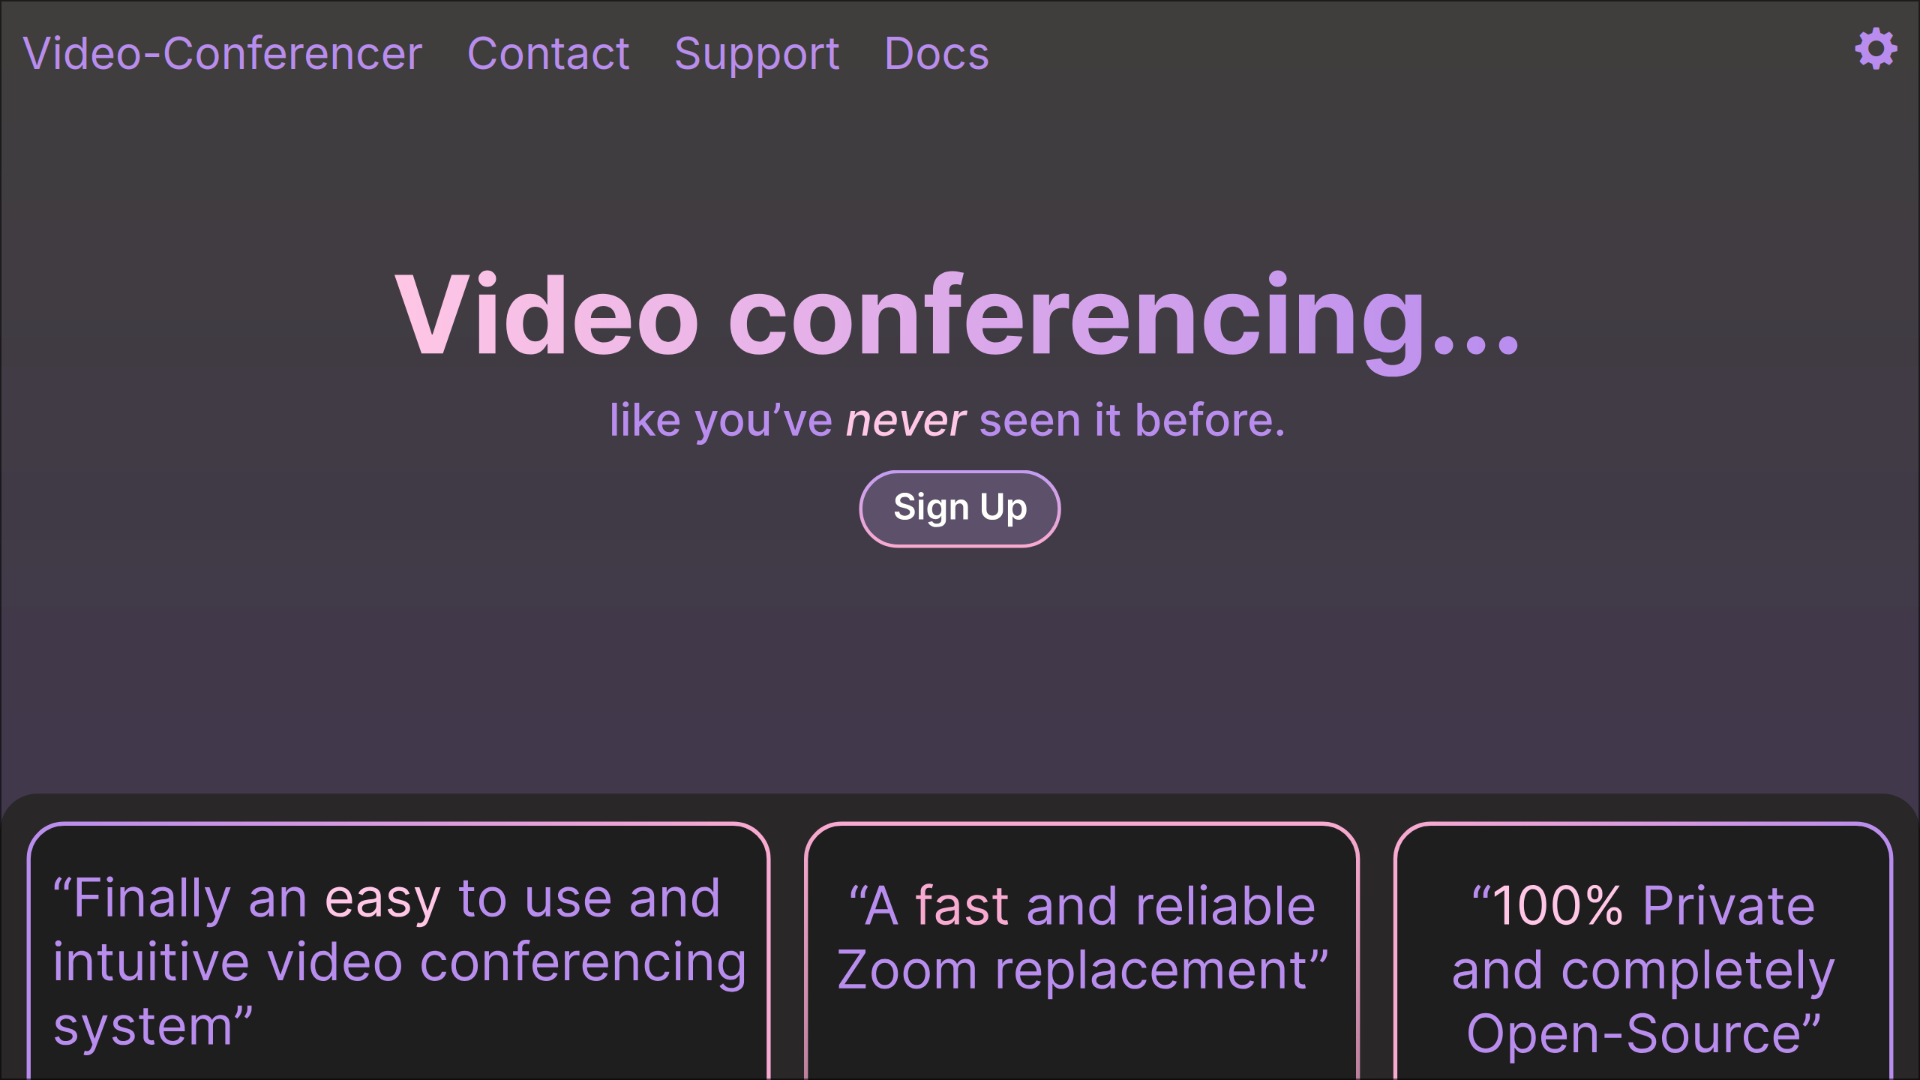
\includegraphics[scale=0.2]{Images/Refined_home.png}

\caption{Refined home page.}
\end{figure}

{\color{gray} \hrulefill} \vspace{0.2cm}

{\sffamily Development sub-task \circled{1} \faCheck}

\subsubsection{Login page}

\textit{Description:} I re-design the login page to fit with the
new theme, and implement my design in HTML and sass.\\ \vspace{0.2cm}

\textit{Explanation and justification:}
Clearly the login page needed to be re-designed also in order
to properly match the theme of the home page. Here is the
revised design for our login page. Inspiration was drawn
from Spline's login UI \url{https://spline.design/}.

\begin{figure}[H]
\centering

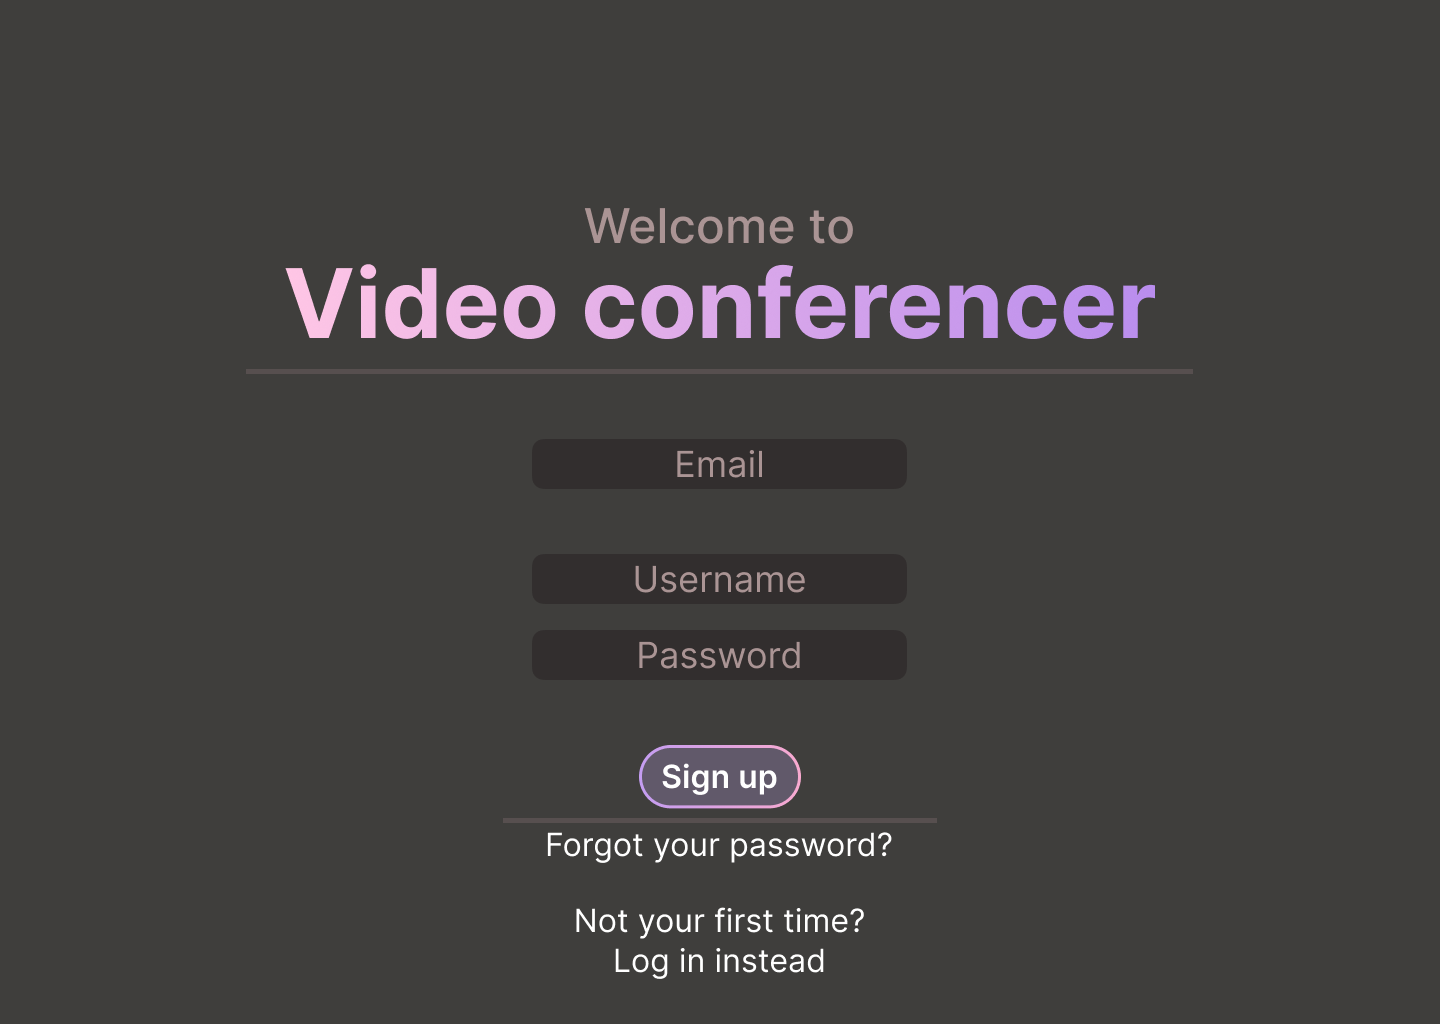
\includegraphics[scale=0.2]{Images/Login_Page_2.png}

\caption{2nd Mock up of the login page.}
\end{figure}

This revised version fits much nicer with the home page.
During the creation of this page however I realised that I
had not yet discussed what we would do if a user had
forgotten their password. In such a case we could employ
the standard technique of sending the user a reset password
link to their email address and I have included this in
our mock up. This idea will have to be added as a development
sub-task and we will tackle it's implementation in a future
iteration. \\ \vspace{0.2cm}

The next step is to transfer the design in code, then link
our home page and login page together. During the programming
of the home page I realised that I would be using the same
sign-up button design as the one designed on the home page.
Recalling that I would apply the DRY
("\textbf{D}on't \textbf{r}epeat \textbf{y}ourself") principle
whilst I wrote my code (see section \ref{sec:computational}),
I decided to put the button code in it's own file
\texttt{button\_styling.sass} and simply have the other \texttt{.sass}
files import from the button styling file whenever needed. Now
that I had gained some experience with translating my designs into
HTML and CSS I was able to make some changes to the design on the
fly to improve upon the figma mock up design. \\ \vspace{0.2cm}

\underline{login.html}

\begin{minted}[linenos, bgcolor=lightestgray]{html}
...
<body>

  <object id="Headline" data="Images/Welcome.svg" type="image/svg+xml">
    <img src="Images/Welcome.png">
  </object>

  <center>
    <b id="Login_Prompt"> Log in instead? Click here </b>
  </center>

  <br><br>

  <center>

    <div id="Login">

      <form>
	<input type="text" placeholder="Email" name="email" required>       <br><br><br>
	<input type="text" placeholder="Username" name="username" required> <br><br>
	<input type="password" placeholder="Password" name="password" required autofocus>
	<br> <br> <br>

	<button class="Button"> <b> Sign up </b> </button> <br><br>

	<div class="Rule"> </div> <br>

	<p style="color:white; font-size: 20px"> Forgot your password? </p>
      </form>
    ...
\end{minted}

\underline{styles\_login.sass}

\begin{minted}[linenos, bgcolor=lightestgray]{sass}
@use './button_styling.sass'
@import url('https://fonts.googleapis.com/css?family=Inter')
@import url('https://maxcdn.bootstrapcdn.com/bootstrap/3.3.7/css/bootstrap.min.css')

// Colour definitions
...

// Setting font and background colour
body
  height:           100vh
  margin:           0
  background-color: $Col_Main
  ...

.Rule
  width: 40%
  border-bottom: 4px solid $Col_Rule

// Positioning the headline
#Headline
  display:      block
  margin-left:  auto
  margin-right: auto
  ...

// Positioning the login box
#Login
  disply:       block
  margin-left:  auto
  margin-right: auto

// Styling the input field
input
  border-radius:    12px
  width:            281px
  height:           37.5px
  ...

#Login_Prompt
  color:     white
  font-size: 20px
\end{minted}

This code produced our first prototype:

\begin{figure}[H]
  \centering
  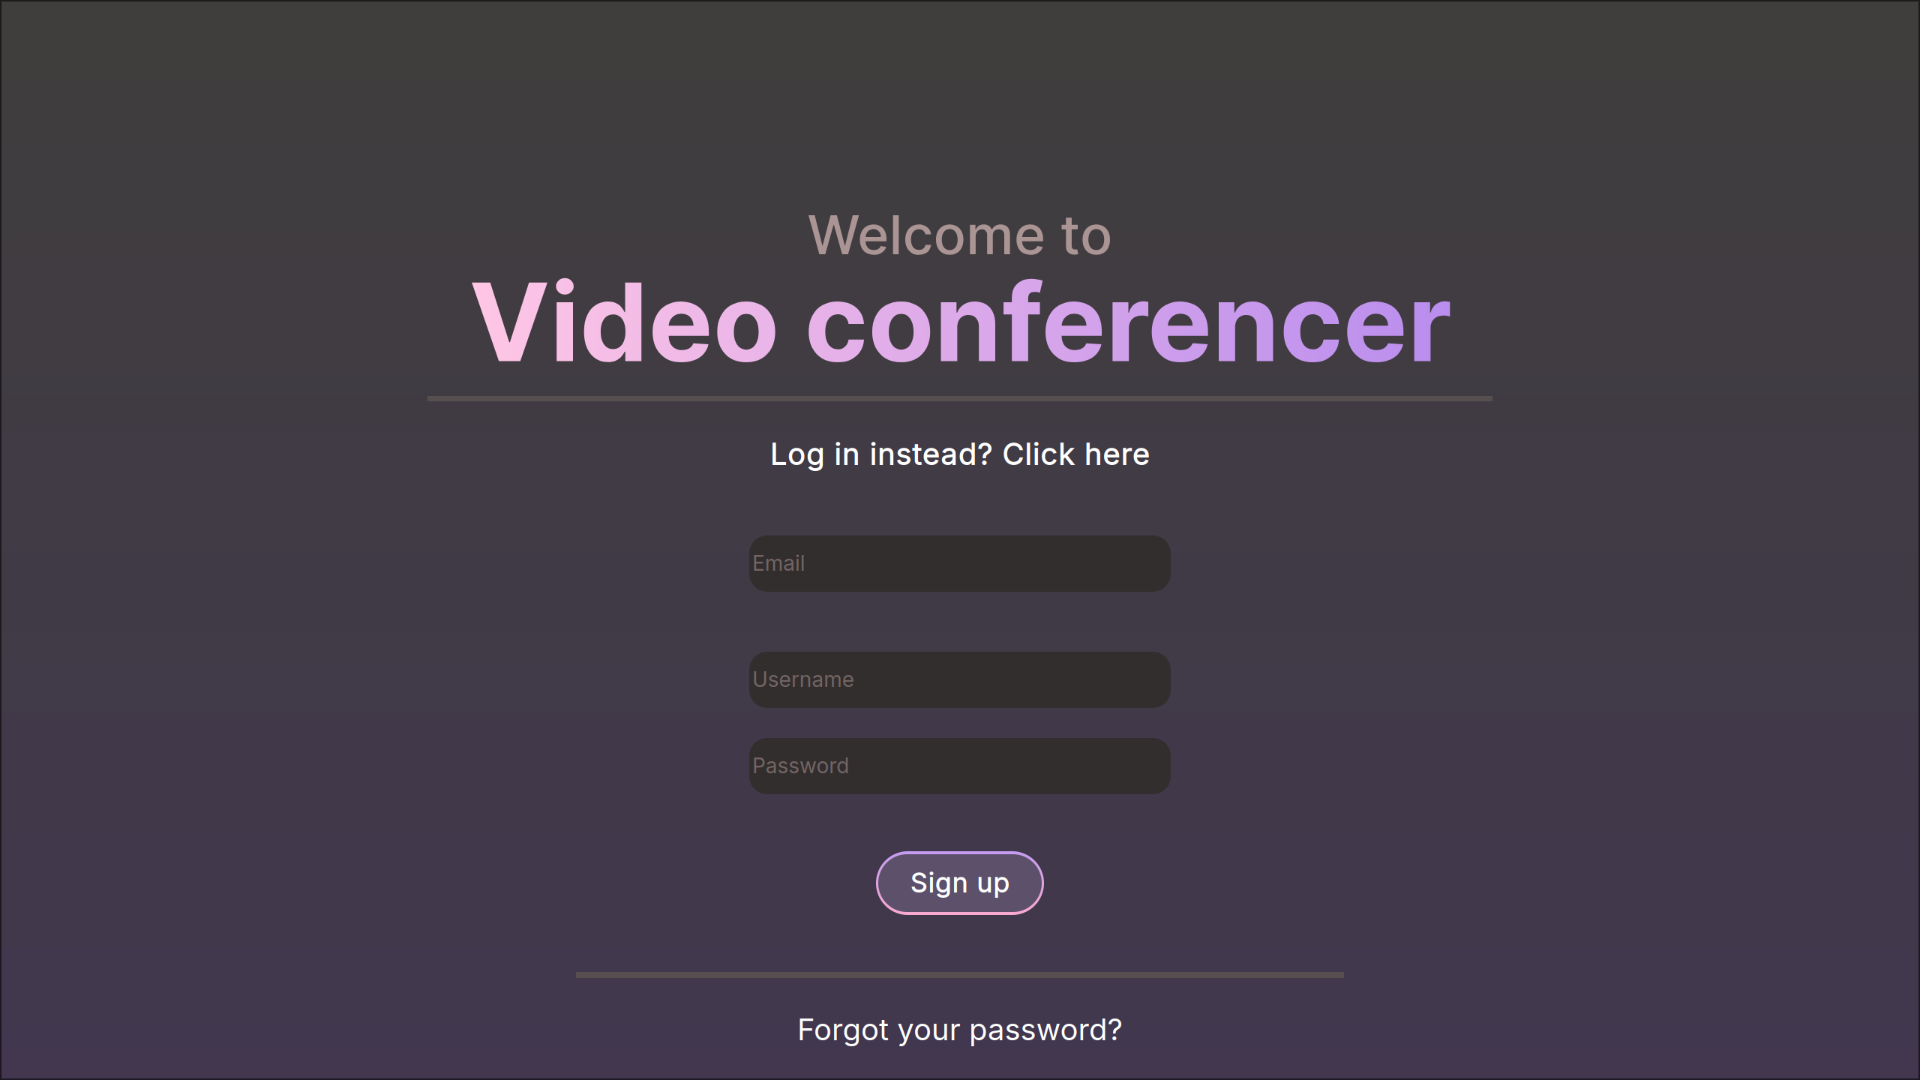
\includegraphics[scale=0.2]{Images/LoginUI.png}
  \caption{Login UI prototype 1}
\end{figure}

{\color{gray} \hrulefill} \\ \vspace{0.2cm}

{\sffamily Client feedback:}

\begin{itemize}
  \item Looks great!
\end{itemize}

{\color{gray} \hrulefill}
\vspace{0.2cm}

{\sffamily Development sub-task \circled{1.2} \faCheck} \\
\vspace{0.2cm}

Look at Github commit
\texttt{54e06ac60f0876086c259f29ce23eae89ff4aad6} to
see the state of the project after our first iteration.\\
\vspace{0.1cm}

Alternatively click the following link to view the state of
the project at this point in development: \\
\href{https://github.com/zzzNathan/Video-Conferencer/tree/54e06ac60f0876086c259f29ce23eae89ff4aad6}{
\texttt{VideoConferencer-Iteration1}}.

\section{Iteration 2}

During this iteration I wanted to design and implement
some of the underlying infastructure behind our application
and complete development subtasks \circled{2} and \circled{A}.\\
\vspace{0.2cm}

\textit{Description:}
After doing some of research into free web deployment
services I settled on using Vercel in order to deploy my website.\\
\vspace{0.2cm}

\textit{Explanation and justification:}
Here are a few of the other options I looked into and why I rejected
them. \\ \vspace{0.2cm}

\begin{tblr}{colspec={XX}, row{1}={lightestgray}}
Service & Explanation \\

Railway.app & You can only use \$5.00 worth of resources on the
free tier, once this is depleted the project won't be up
anymore \\

render.com & Projects on the free tier are deleted automatically after 1 month \\
\end{tblr}

On the other hand Vercel doesn't have any of these drawbacks, so my
site will be able to stay up permanently so long as some resource limits are
not crossed. \\ \vspace{0.2cm}

\textit{Description:} In order to use Vercel to deploy my web
application I had to use a web framework. I chose to use React with
Vite and rewrote my existing codebase to work with this framework. \\
\vspace{0.2cm}

\textit{Explanation and justification:}
Initially I intended to try and stay away from all of these
web-frameworks and just stick to plain old HTML and CSS (or
sass in our case), however an issue arose when I wanted to
redirect users to our registration page once they clicked
the sign up button on our home page. For whatever reason
the redirection would work when I hosted the application on
my own machine, however when I would deploy to vercel the
redirection would either, simply not change page or display
a 404 code not found error.

\begin{figure}[h]
\centering

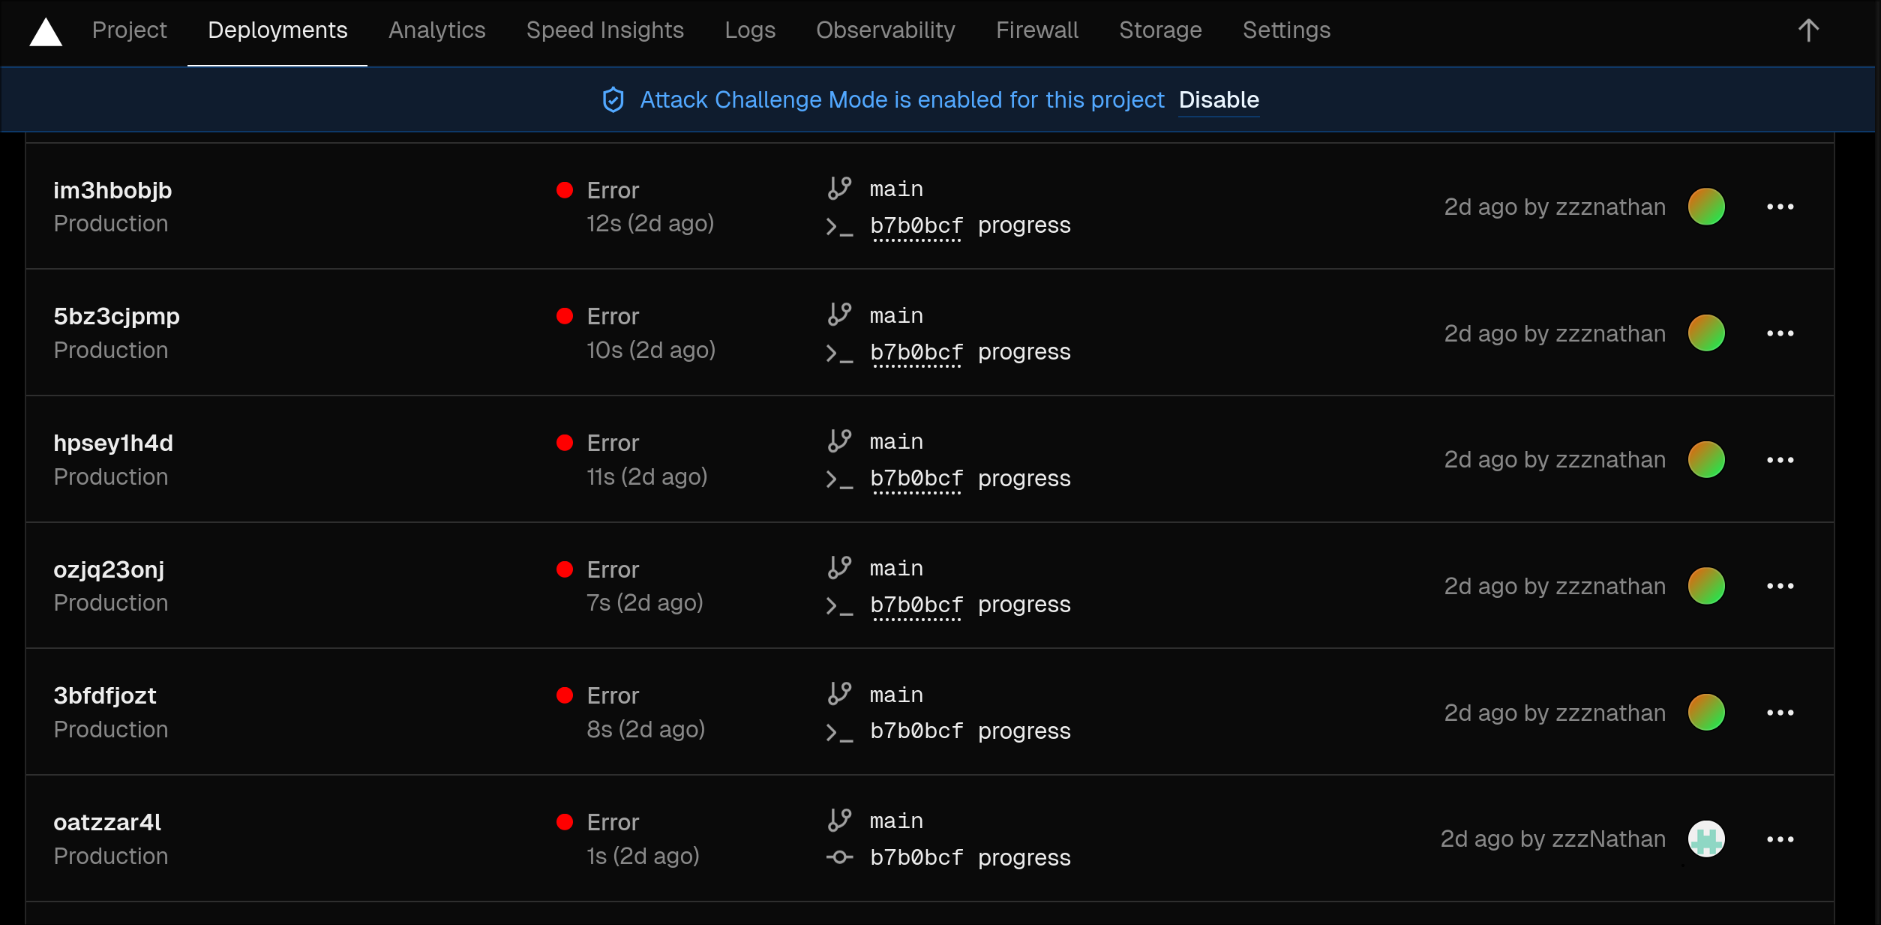
\includegraphics[scale=0.2]{Images/Vercel_Errors.png}

\caption{Errors when deploying to Vercel.}

\end{figure}

Eventually after a lot of trial and error and some research,
I found out that using a router with react would allow us to
redirect the user to different pages once deployed. I then
took some time to migrate our codebase to JSX to work with the
react framework. We will omit the code for the re-written
webpages since it is pretty similar to the snippets shown in
Iteration 1. Here is what the routing logic looks like. \\
\vspace{0.2cm}

\underline{main.jsx} \\ \vspace{0.2cm}

\begin{minted}[linenos, bgcolor=lightestgray]{jsx}
import { createRoot } from "react-dom/client"
import { createBrowserRouter, RouterProvider } from "react-router-dom"
import Home from "./components/Home.jsx"
import Registration from "./components/Registration.jsx"

// Path is an extension that goes after our URL,
// once this extension is written the corresponding
// React element will be loaded and rendered.
const router = createBrowserRouter([
  {
    path: "/",
    element: <Home />
  },
  {
    path: "/registration",
    element: <Registration />
  }
])

createRoot(document.getElementById('root')).render(
  <RouterProvider router={router} />
)
\end{minted}

\textit{Description:} I used the Clerk user management
platform to create a user account registration form.\\
\vspace{0.2cm}

\textit{Explanation and justification:} I originally wanted to
do this task manually, creating my own table and then querying
this table in order to add new users and log users in. However
after doing some reading and looking over Stack Overflow posts
like this one \url{https://stackoverflow.com/questions/46819734/how-to-check-username-and-password-matches-the-database-values}
I realised that many issues can arise when developers try to
implement these systems themselves. In order to avoid this
plethora of issues I instead chose to use the Clerk.com API
\footnote{I originally came across this API watching Theo T3.gg's
React tutorial.}
for user authentication. Not only was it much easier to implement
but the usage of this API also ensures that I wont have to worry
about any security issues, since the API has been thoroughly
tested. Here's the implementation. \\ \vspace{0.2cm}

\underline{Registration.jsx}
\begin{minted}[linenos, bgcolor=lightestgray]{jsx}
import { ReactTyped } from "react-typed"
import { ClerkProvider, SignedOut, SignUp } from "@clerk/clerk-react"
import { dark } from "@clerk/themes"
import Navbar from "./Navbar"
import "../styles/Registration.sass"

const PUBLISHABLE_KEY = import.meta.env.VITE_CLERK_PUBLISHABLE_KEY
...

function Registration () {
  return (
  <> <Navbar />
    <Headline />

    <ClerkProvider publishableKey={PUBLISHABLE_KEY}>
      <SignedOut>
        <center> <SignUp appearance={dark}/> </center>
      </SignedOut>
    </ClerkProvider>
  </>
  )
}

export default Registration
\end{minted}

Here is what the code renders to:

\begin{figure}[H]
\centering

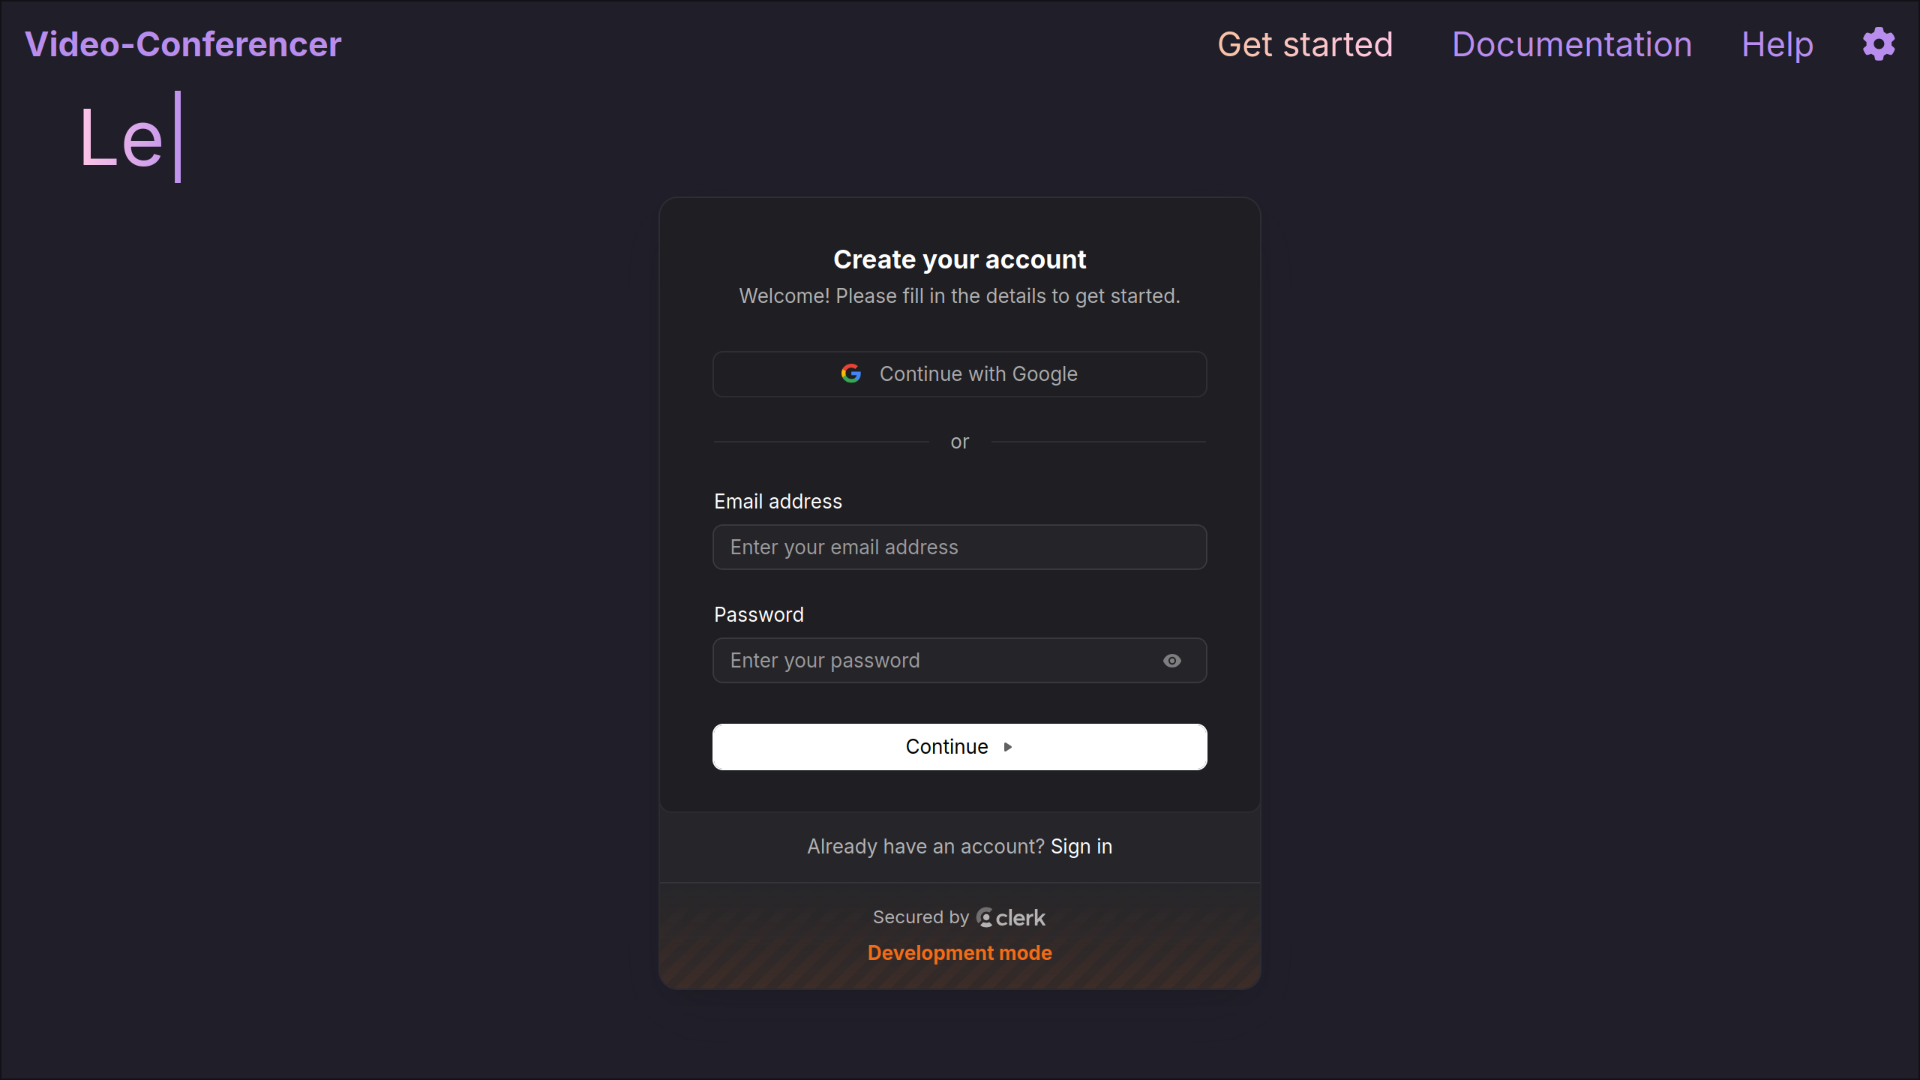
\includegraphics[scale=0.2]{Images/Registration.png}

\caption{Rendering the registration page.}
\end{figure}

{\color{gray} \hrulefill}
\vspace{0.2cm}

{\sffamily Tests:}
\begin{itemize}
  \item Site home page loads correctly \faCheck \\
  \item Correctly redirected to registration page \faCheck \\
  \item Users can create a new account \faClose \\
\end{itemize}

{\sffamily Evidence: \url{https://youtu.be/tHUQeArAv-g}}

{\color{gray} \hrulefill}
\vspace{0.2cm}

The reason why the registration page wasn't rendering was because
I made use of Clerk's \code{useUser()} function in my
\code{<Navbar />} component outside of a ClerkProvider component.
As per the documentation \textit{"The}
\code{<ClerkProvider>} \textit{component is required to integrate
Clerk into your React application, providing session and user
context to Clerk's hooks and components."}
\footnote{Source: https://clerk.com/docs/components/clerk-provider}
This makes sense since
the Clerk SDK would need to have context about the current user
logged in order to get the information returned in the
\code{useUser()} hook, like the \code{user.id} and the
\code{user.username}. \\ \vspace{0.2cm}

This issue was fixed by simply wrapping my HTML code in the
\code{<ClerkProvider>} component whenever a page made usage of the
\code{<Navbar />}. All the tests now successfully pass. \\ \vspace{0.2cm}

Note that with this we have achieved success criteria 5 and 6. \\ \vspace{0.2cm}

{\color{gray} \hrulefill}
\vspace{0.2cm}

{\sffamily Tests:}
\begin{itemize}
  \item Site home page loads correctly \faCheck \\
  \item Correctly redirected to registration page \faCheck \\
  \item Users can create a new account \faCheck \\
\end{itemize}

{\sffamily Evidence: \url{https://youtu.be/IjwQH1Z8aPw}} \\ \vspace{0.2cm}

{\sffamily Input Validation:}
\begin{itemize}
  \item Site doesn't allow users to input weak passwords \faCheck \\
  \item Site doesn't allow users to input email addresses that aren't of the correct format \faCheck \\
\end{itemize}

{\sffamily Evidence: } \url{https://youtu.be/p-rWgn692KU}

{\color{gray} \hrulefill}
\vspace{0.2cm}

You can try these features out yourself at \url{https://video-conferencer.vercel.app/registration}.
(May not work if development is ongoing).\\ \vspace{0.2cm}

{\sffamily Development sub-task \circled{2} \faCheck \\ \vspace{0.2cm}
Development sub-task \circled{A} \faCheck } \\ \vspace{0.2cm}

Look at Github commit \texttt{243560c390c019ab39903850ef3dba99ed98df18} to see the state of the project after our first
iteration. \\ \vspace{0.2cm}

Alternatively click the following link to view the state of
the project at this point in development: \\
\href{https://github.com/zzzNathan/Video-Conferencer/tree/243560c390c019ab39903850ef3dba99ed98df18}{
\texttt{VideoConferencer-Iteration2}}.

\newpage

\section{Iteration 3}

During this iteration I wanted to further develop the backend
infastructure of our application, and start to sketch out the
actual implementation for including video conferencing in our
application. I also improve the code and touch up some of the
designs, and use Clerk to rewrite the login page. With that
we implement tasks \circled{8} and \circled{B} \\ \vspace{0.2cm}

\textit{Description:} I rewrite the login page using clerk,
and make minor improvements to our landing page. \\
\vspace{0.2cm}

\textit{Explanation and justification:} Our users can now
register an account with Clerk, so they will also have to
login using the Clerk SDK aswell. During this time I also
improved the landing page design. These improvements
contribute to the professional look and feel of our website
and enhance the user experience. \\ \vspace{0.2cm}

\underline{Login.jsx}

\begin{minted}[linenos, bgcolor=lightestgray]{jsx}
...
// Makes the typing headline animation
function Headline ()
{
  return (
    <ReactTyped
      className={"Headline"}
      strings={[
        "Welcome back :)",
	"    Log back in here,",
      ]}
      typeSpeed={120}
      startDelay={30}
      loop
    >
    </ReactTyped>
  )
}

// Renders the login page
function Login () {
  return (
  <>
    <ClerkProvider publishableKey={PUBLISHABLE_KEY}>
      <Navbar />
      <Headline /> <br/>
      <SignedOut> <center>

        <SignIn
          signUpUrl="/registration"
          forceRedirectUrl="/home"
          appearance={{
            baseTheme: dark,
            variables: {spacingUnit: "2vh"}
	  }}
	/>

      </center> </SignedOut>
    </ClerkProvider>
  </>
  )
}

export default Login
\end{minted}

Here's what the code renders to: \\

\begin{figure}[H]

\centering
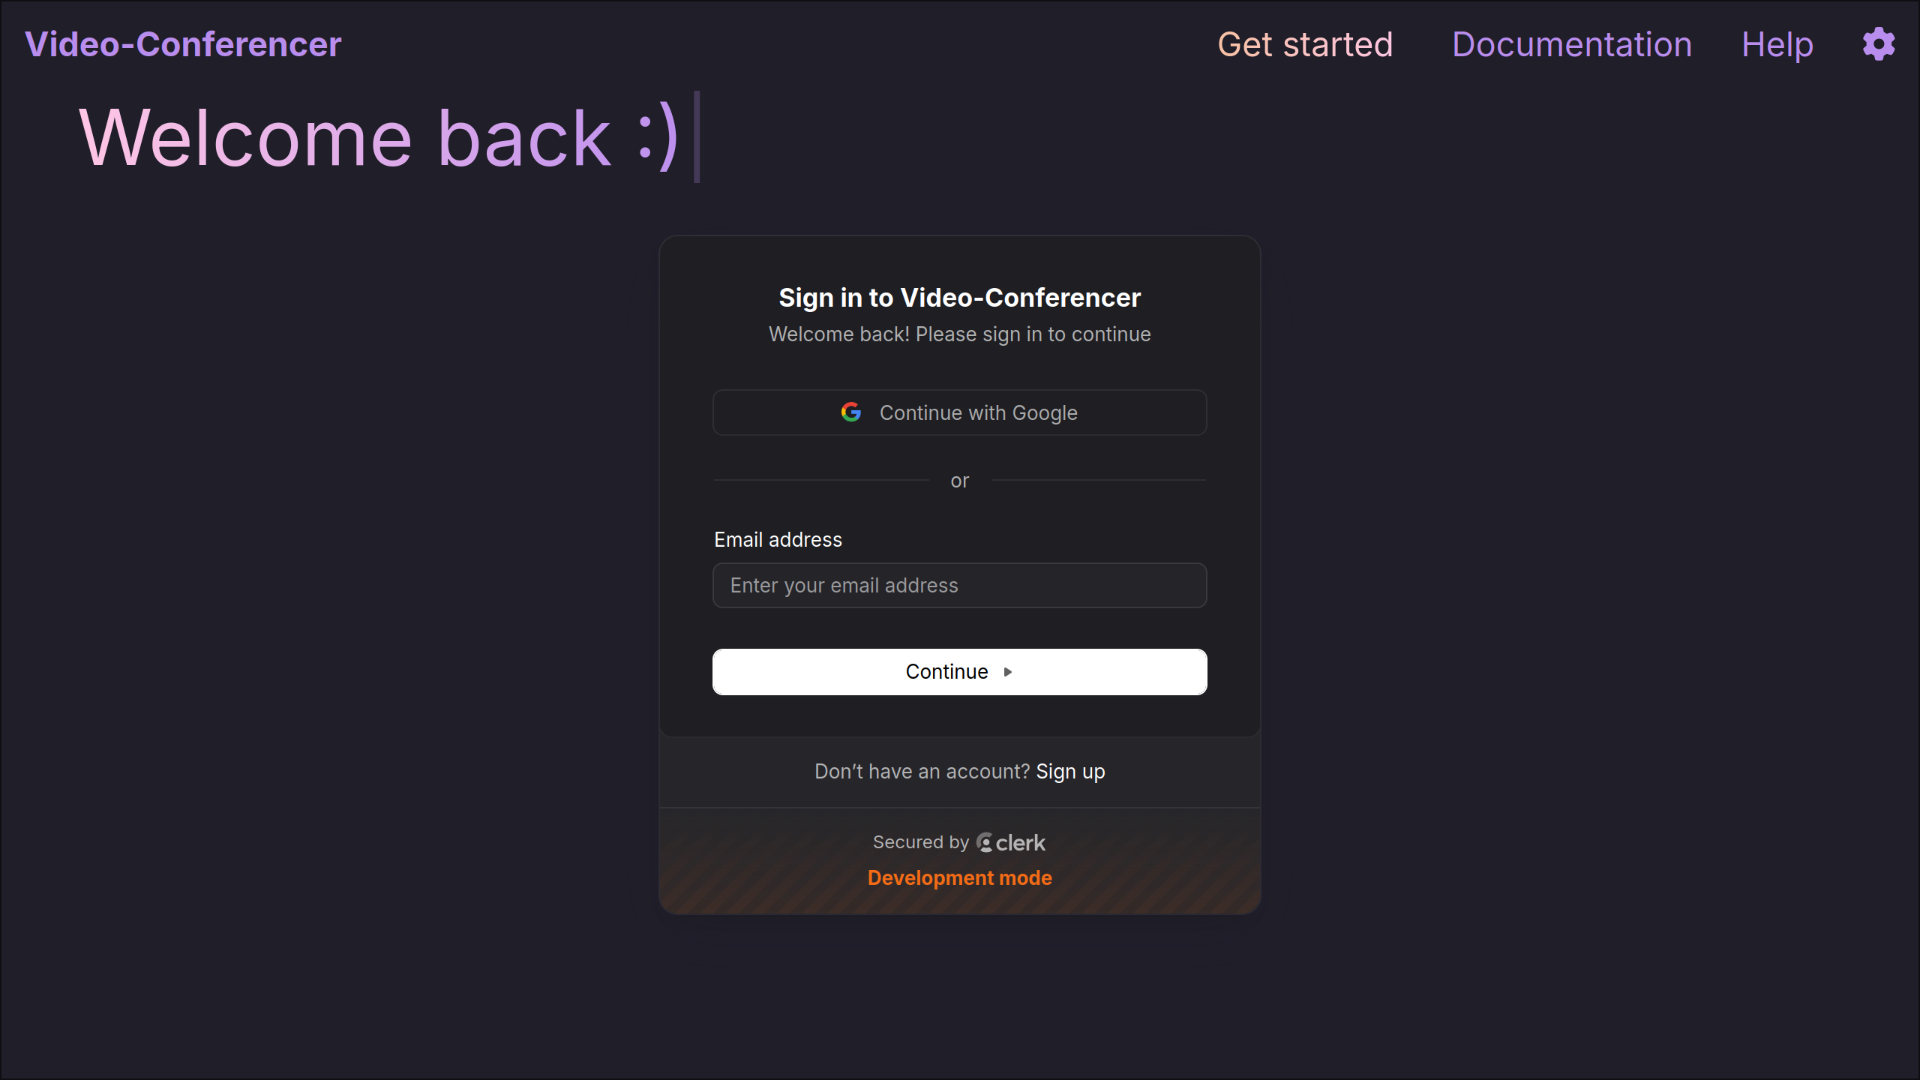
\includegraphics[scale=0.2]{Images/Login.png}

\caption{Rendering the login page.}

\end{figure}

\textit{Description:} I design and implement the page that
users will see after logging in to their account. \\
\vspace{0.2cm}

\textit{Explanation and justification:} In order to start,
join video conferences and change video configuration
settings, the user must have some way to be able to access
these features. The UI should allow our users to easily
navigate the site, providing a good user experience whilst
still looking professional. I began by making a quick sketch
of the design I had in mind. \\

\begin{figure}[h]
\centering

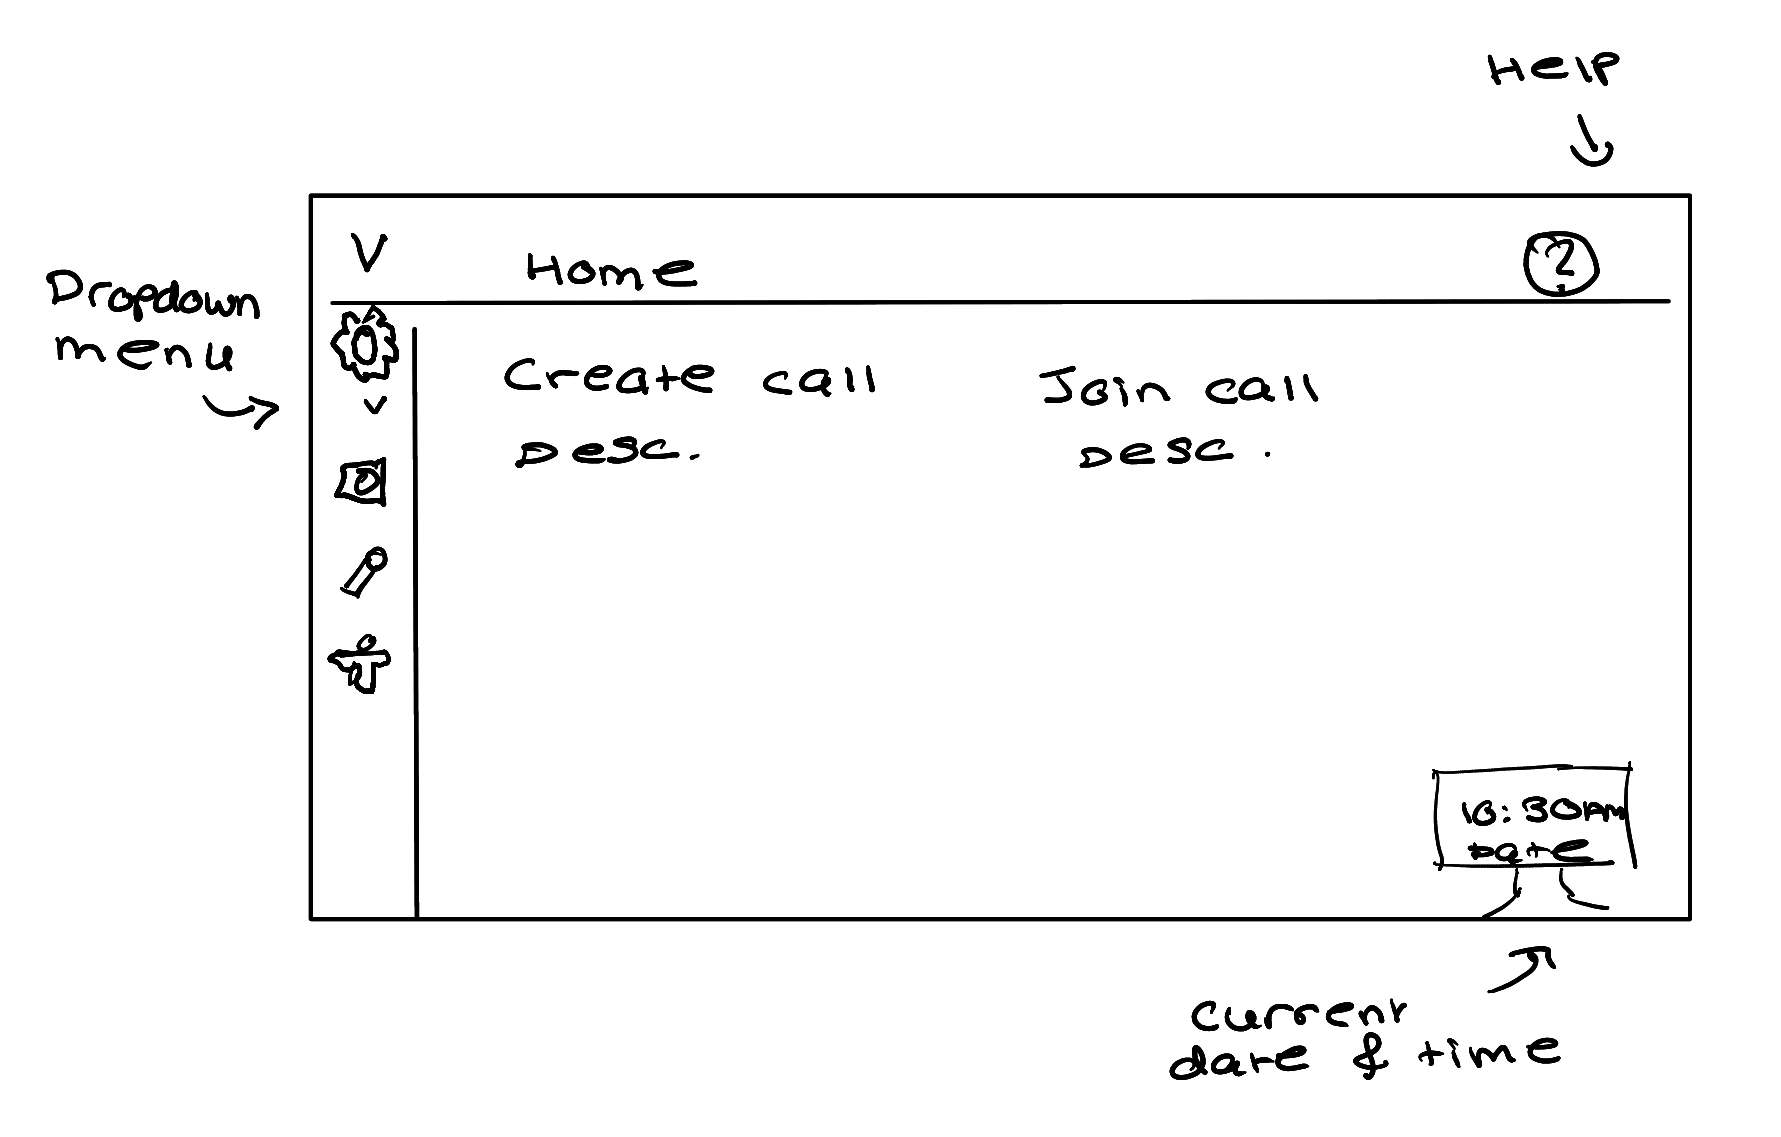
\includegraphics[scale=0.2]{Images/Home_sketch.png}

\caption{Sketching out the design.}
\end{figure}

From here it was pretty simple to write out the code to make
this UI. \\ \vspace{0.1cm}

\textit{Confusingly from here on we call this page
our home page and the page previous home page our landing
page in our code base. In this document we will use the
following names. We will call the page that the user first
sees our 'home' page, we will call the page that the user
first sees after logging in our 'main' page.} \\
\vspace{0.2cm}

\underline{Home.jsx}

\begin{minted}[linenos, bgcolor=lightestgray]{jsx}
import "../styles/Home.sass"
import Clock from "./Clock.jsx"
...

function Options () {
  const Create_Desc = <div className="Desc">
    Create a new video call, then invite others
    to join by giving them the call code given
    to you once you start the call.
  </div>

  const Join_Desc = <div className="Desc">
    Enter the code given to you to join the
    video call.
  </div>

  return (
    <ul className="Options">
      <li> Create call <br/> {Create_Desc} </li>
      <li> Join call   <br/> {Join_Desc}   </li>
    </ul>
  )
}

function Home () {
  return (
    <> <Top_Bar />
    <Side_Bar />
    <Options />

    <Clock />
    </>
  )
}

export default Home
\end{minted}

\begin{figure}[H]
\centering

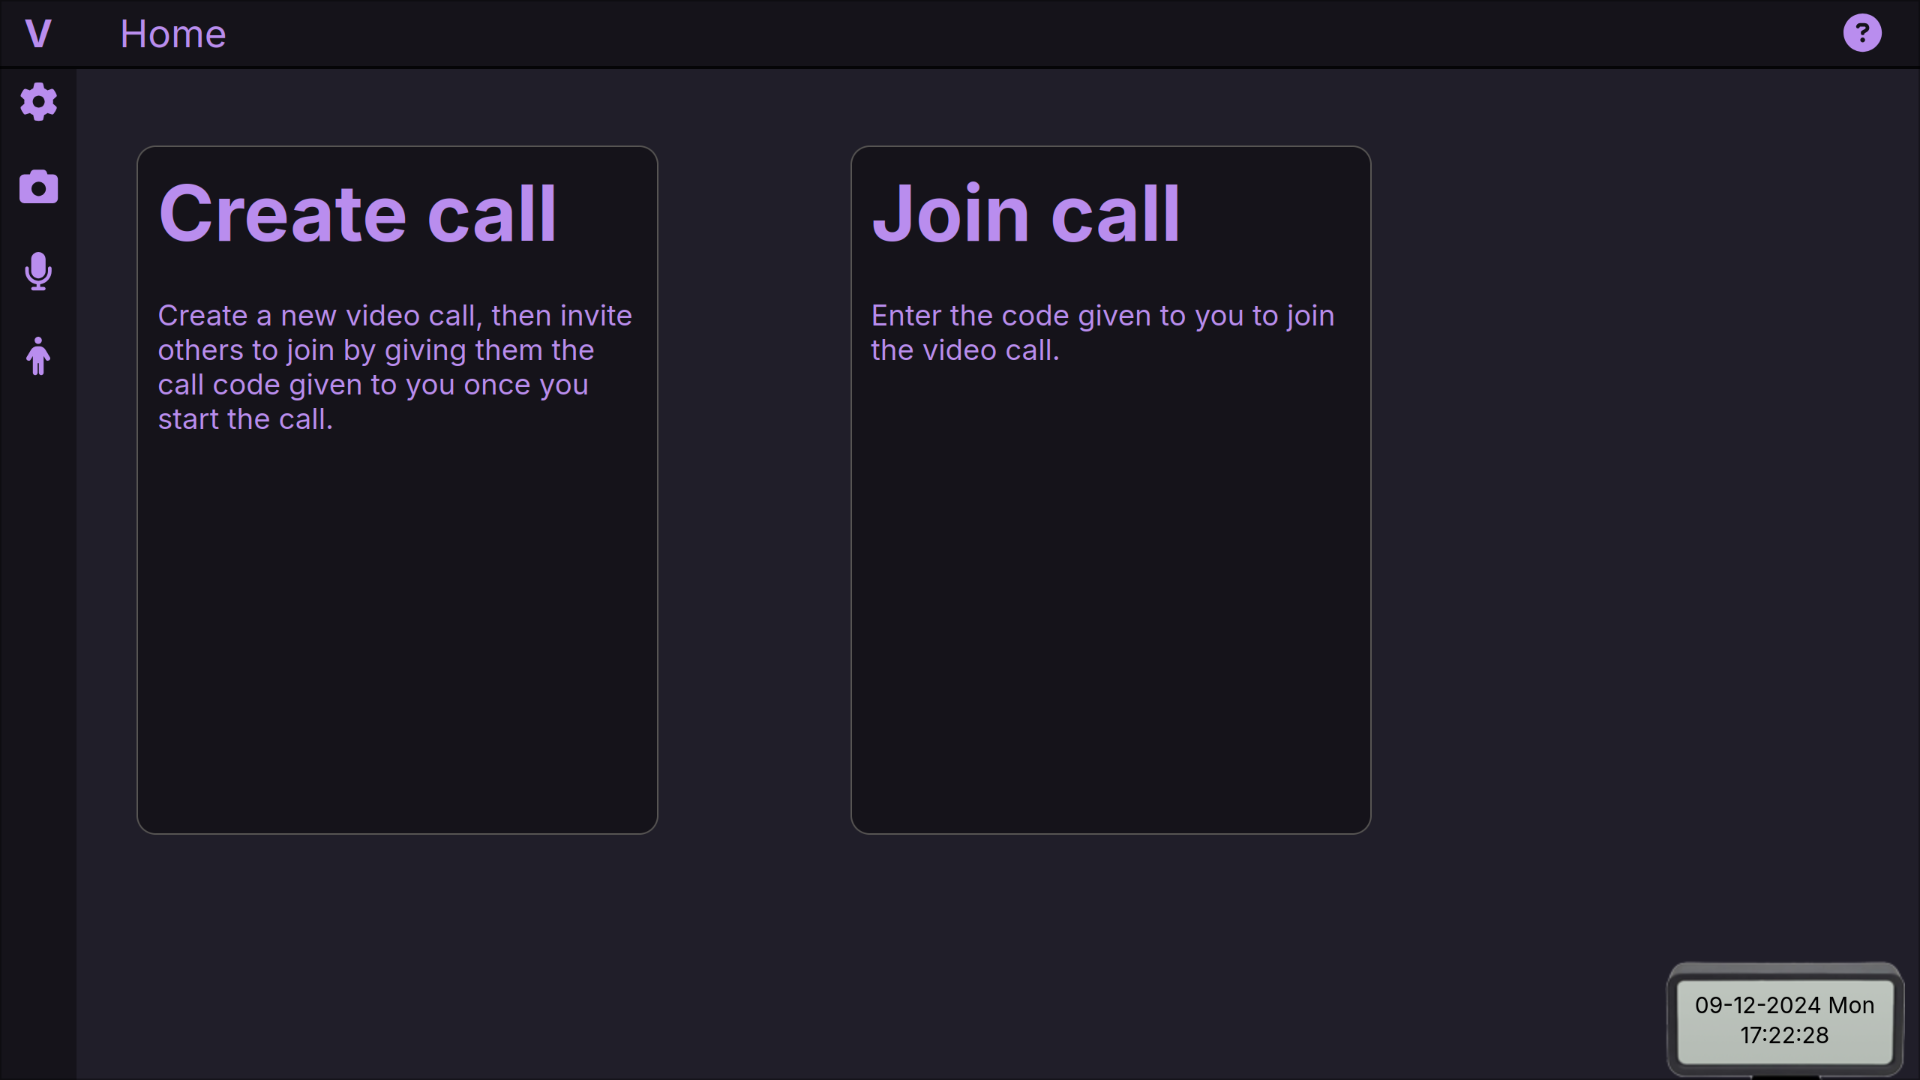
\includegraphics[scale=0.2]{Images/Sketch_final.png}

\caption{Implementing the code for the sketch.}
\end{figure}

\textit{Description:} I chose to use the GetStream React
library to implement video conferencing in my application. \\
\vspace{0.2cm}

\textit{Explanation and justification:} As detailed in my research, I first
intended to use the WebRTC framework provided by Google to
write the video conferencing logic. However after some research
into what it would take for me to implement such a system I
realised that actually implementing the logic would take me
an unreasonable amount of time. Taking into consideration the
fact that I would have to understand and correctly implement
the sending of SDP protocol offers, connecting each user to a
STUN server, whilst ensuring that each user has access to
the other user's ICE candidates, the task felt as though it
would take me a number of weeks to implement such a system
to allow 2 users to video conference properly, let alone have
$n$ users video conference simaltaenously. So instead I chose
to use a popular industry standard video conferncing library
called GetStream. \\ \vspace{0.2cm}

The first step to have users be able to
video conference was to have our users be authenticated as
users on the GetStream API. According to the documentation
in order to do this each user must be given a unique JWT
(JSON web token) token via GetStream's
\code{client.generateUserToken()} function. In the documentation
it explicitly says \textit{"Tokens need to be generated server-side,
... You need to implement the token provider in your own application,
this is usually an HTTP endpoint."} \footnote{Source:
\url{https://getstream.io/video/docs/api/authentication/}}
In order to run the backend code I would need a server or some
other place to be able to host my code. After reading through
some forums online I came across Cloudflare's Worker service.
This service allows users to be able to run server side code
remotely through one of Cloudflare's many servers across the globe,
with pretty generous free tier limits. I quickly set up an account
with Cloudflare and began to implement my HTTP API. \\ \vspace{0.2cm}

\underline{/backend/stream-token-provider/src/index.js} \\

\begin{minted}[linenos, bgcolor=lightestgray]{js}
...

// An HTTP endpoint that allows POST requests
// with a user id given in the request. Will return
// a unique user token that can be used to begin
// video conferencing
async function Provide_Token(request, env)
{
  const { method } = request;

  // Ensure that the request is a POST
  if (method !== 'POST')
    return new Response('Method not allowed', { status: 405 });

  try {
    const { User_Id } = await request.json();

    // Ensure that a valid user id is actually provided
    if (!User_Id || User_Id.length != USER_ID_LENGTH)
      return new Response('Bad Request: Proper userId is required', { status: 400 });

    const apiKey = env.STREAM_API_KEY;
    const secret = env.STREAM_API_SECRET;

    const token = await Generate_Token(User_Id, apiKey, secret);

    return new Response(JSON.stringify({ token }), {
      headers: { "Content-Type": "application/json" },
    });

  } catch (error) {
      return new Response(`Error: ${error.message}`, { status: 500 });
  }
}
...
\end{minted}

{\color{gray} \hrulefill} \\ \vspace{0.2cm}
{\sffamily Tests:}

\begin{itemize}
  \item HTML endpoint is accessible \faCheck \\
  \item Only POST requests are allowed \faCheck \\
  \item A GetStream token is actually provided in the output \faCheck
\end{itemize}

{\sffamily Evidence: \url{https://youtu.be/Ia1knGrbcaE}}

{\color{gray} \hrulefill}
\\ \vspace{0.2cm}

\textit{Description:} I add user id validation to our backend.
\\ \vspace{0.2cm}

\textit{Explanation and justification:} There was no information
to be found on the way that Clerk formats it's user id's, so the
user id validation we can do is quite limited. We simply check
whether or not the string length $s$ satisfies $0 < s \leq 512$.
\\ \vspace{0.2cm}

\begin{minted}[linenos, bgcolor=lightestgray]{js}
...
const MAX_USER_ID_LENGTH = 512
...
// Validate the user id given is correct
function Validate_User_Id(User_Id)
{
  if (User_Id.length > MAX_USER_ID_LENGTH ||
      User_Id.length == 0)
    return false

  return true
}
...
\end{minted}

\textit{Description:} I fix a bug with button misalignment on
mobile. \\ \vspace{0.2cm}

\textit{Explanation:} Whilst testing out how my website works
on different devices, I found that although the page looks
fine on desktop, on mobile the buttons on the home page seem
to be misaligned. \\

\begin{figure}[h]
\centering

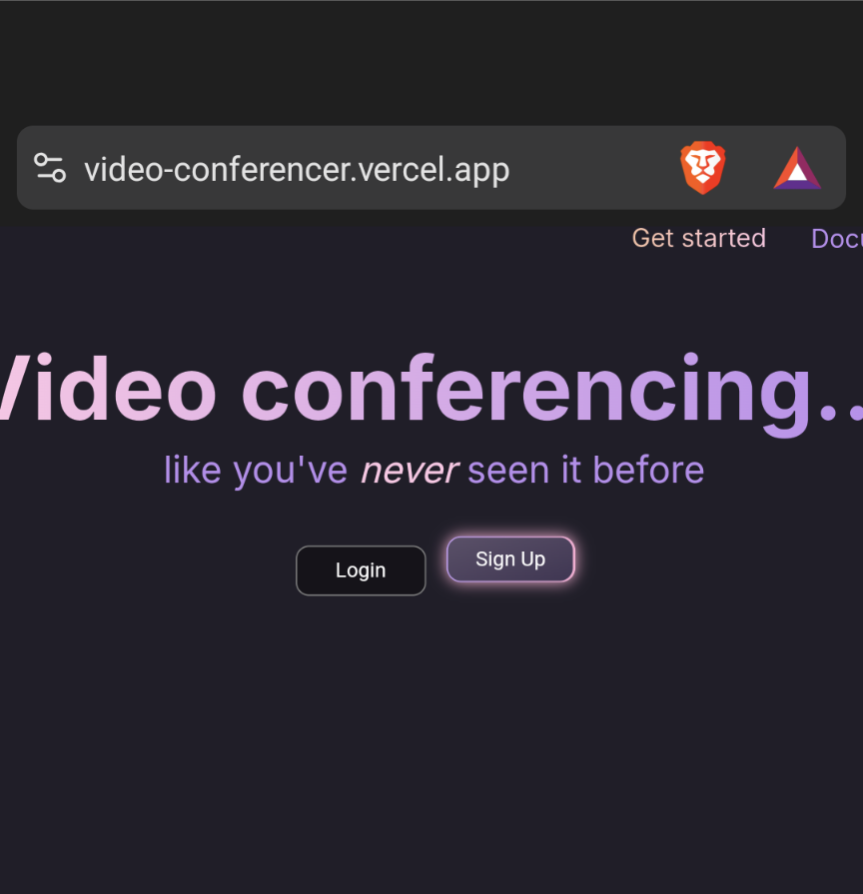
\includegraphics[scale=0.2]{Images/Button_misalignment.png}

\caption{Buttons being misaligned on mobile}
\end{figure}

In order to fix this I simply changed the sass of the login
button to use a pseudo element for it's border, so that it is
created in the same way the sign up button is created. By
doing it this way we can be 100\% sure that both buttons will
now be the same exact size, and that hence we will have no
more alignment issues. \\ \vspace{0.2cm}

\underline{Landing.sass}

\begin{minted}[linenos, bgcolor=lightestgray]{sass}
...
.Login_Button
  border-radius:    0.9vw
  color:            white
  background-color: $Col_Black
  ...

.Login_Button::after
  content:          ''
  position:         absolute
  height:           107%
  ...

.Login_Button:hover
  scale: 104%
...
\end{minted}

These changes fixed our issues with button misalignment.

\begin{figure}[H]
\centering

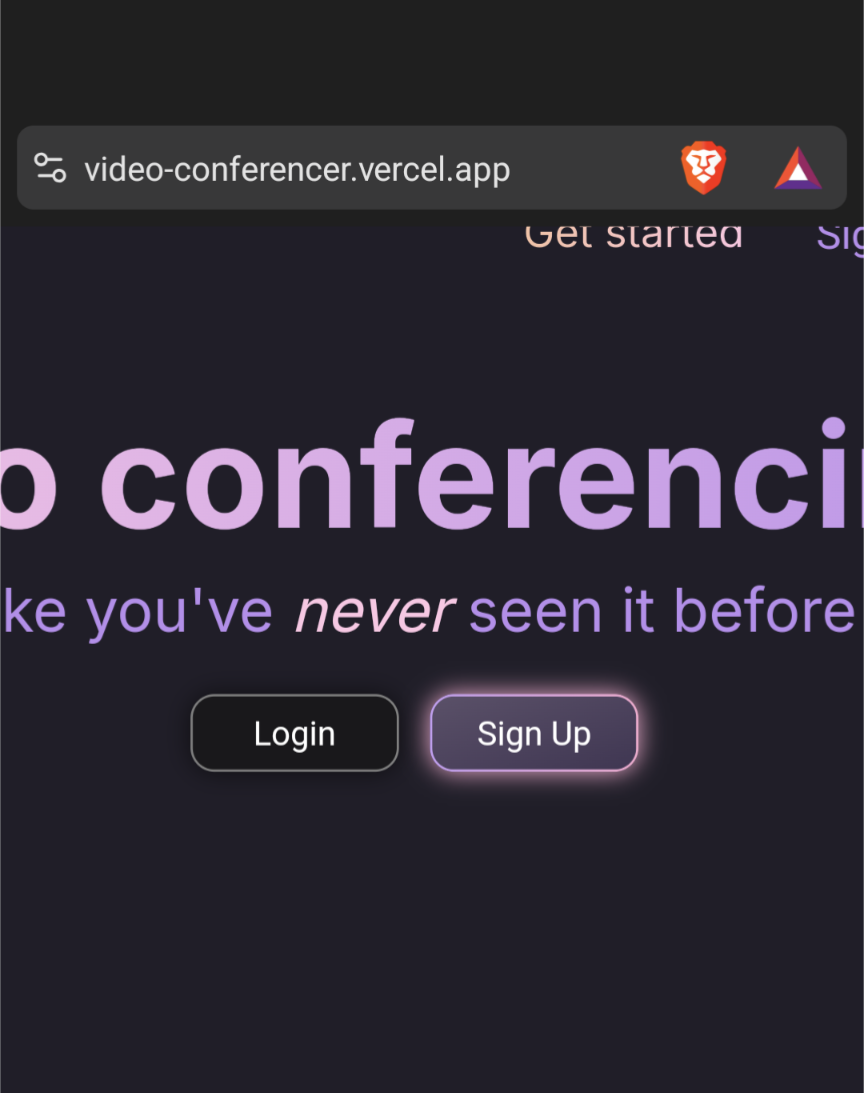
\includegraphics[scale=0.2]{Images/Buttons_aligned.png}

\caption{Buttons being fixed on mobile}
\end{figure}

\textit{Description:} We create another Cloudflare worker to
generate unique call ids. These ids will be used to invite
other users to join one's video conference. \\ \vspace{0.2cm}

\textit{Explanation and justification:} We start by discussing
exactly \textit{how} we are going to generate then distribute
these call ids. As for the format of call ids I decided to
use a 6 digit code \footnote{In reality we exclude the use
of the code \texttt{000000}. This difference is negligable
in our calculations}, providing us with $10^6$ unique call
codes. Note that we can easily increase the number of unique
call codes by allowing ascii characters to used in the call
codes. As users create calls using these ids we would need to
store information in a database to track which call ids are
in use and which call ids are currently available.
\\ \vspace{0.2cm}

An obvious naive algorithm would be to iterate over all call
ids, and individually check whether each one is currently
available. This algorithm would have a worst case time
complexity of $O(n)$ where $n$ is the number of unique call
ids we have, in this case $n = 10^6$. Since each iteration we
are making a call to a database hosted on the cloud, this
could potentially become a pretty time consuming.
\\ \vspace{0.2cm}

One interesting heuristic could be used to optimise the
performance of our current algorithm. Instead of iterating
over we could use a psuedo-random number generator (PRNG) to
\textit{guess} which call ids are currently available. Indeed
as the number of used call ids $k \leq n$ increases the chance
that we successfully randomly generate an available call id
decreases. Let $G$ be the event that we are investigating.
The probability that we successfully guess an available call
id each time is given by,

$$
  Pr(G) = \frac{n-k}{n} = 1 - \frac{k}{n}
$$

Once the database becomes densely populated, this heuristic
becomes more and more unlikely to yield performant results.
\\ \vspace{0.2cm}

Since the heuristic has a higher chance of yielding results
with a sparse database and the naive algorithm runs in
deterministic time, we could combine these 2 algorithms to
extract the best of both worlds. \\ \vspace{0.2cm}

\begin{algorithm}[H]
\caption{Pseudo-code for a call id generation algorithm.}
\sffamily

\begin{algorithmic}[1]
  \Function{Generate\_Call\_Id}{}
    \Let{Taken}{Number of taken call ids}
    \Let{Total}{$10^6$}

    \State{}

    \If {Taken $/$ Total $\leq 0.25$}
      Generate\_PRNG()
    \EndIf

    \State{}

    \State{\textbf{else} Generate\_Linear()}

  \EndFunction
\end{algorithmic}
\end{algorithm}

\mdseries

When getting into the details of implementing this algorithm
in our backend, since we were already using Cloudflare workers
I decided to make use of Cloudflare's D1 database service to
host our database on the cloud. I wrote a function
to make the implementation of our algorithm go smoother. The
utility function I wrote was the \code{Count\_Elements()} function.
It is a function written to count the number of call ids
currently in use and has an optional arguement \texttt{id}, if
an integer \texttt{id} is provided the function will instead
count the number of call ids in our table with a value of
\texttt{id}. For example if I make the call
\code{Count\_Elements(23)} the function returns the number of
records whose \texttt{id} is 23 in our table. The implementation
is as follows,

\begin{minted}[linenos, bgcolor=lightestgray]{js}
...
// Function to count the number call ids in use
// If the id arguement is passed in then function will
// count the number of call ids equal to the arguement
async function Count_Elements(env, id = null)
{
  var query = `SELECT COUNT(id) FROM ${TABLE_NAME}`

  // If id arguement is passed return the number of ids
  if (id !== null) query += ` WHERE id = ${id}`

  const result = await env.DB.prepare(query).run()

  // Get count from JSON format
  const count = result.results[0]["COUNT(id)"]

  return count
}
\end{minted}

{\color{gray} \hrulefill} \\ \vspace{0.2cm}

{\sffamily Tests:}

\begin{itemize}
  \item HTTP endpoint is accessible \faCheck \\
  \item Function successfully returns the number of call ids in use \faCheck \\
  \item Function successfully returns the number of call ids in use where \texttt{id} is a given value \faCheck \\
\end{itemize}

{\sffamily Evidence:} \url{https://www.youtube.com/watch?v=piCR-SANG3o}\\ \vspace{0.2cm}

{\color{gray} \hrulefill} \\ \vspace{0.2cm}

Next I proceeded to write the \code{Generate\_PRNG()}
function. In Javascript there is no built-in function to
generate a random integer in a given interval rather we
are only provided with the \code{Math.random()} function
which generates a floating point number $n \in [0, 1)$.
We now derive a formula for generating a random integer
number using the built-in random function from JS. \\ \vspace{0.2cm}

Let the \code{Math.random()} function be modelled by
the uniformly distributed continous random variable
$X \in [0, 1)$. Indeed by considering the expression
$cX, (c \in \mathbb{N})$ we can see that the
expression will now lie in the interval $[0, c)$. Then by
applying the floor function
$\left \lfloor {cX} \right \rfloor$ we can force
$\left \lfloor {cX} \right \rfloor \in \mathbb{Z}_{\geq 0}$
or more precisely
$\left \lfloor {cX} \right \rfloor \in [0, c-1]$. We have
made some progress however we don't want to have our lower
bound be 0, we want it to be 1 (see the previous footnote).\\
\vspace{0.2cm}

It is often the case in math, that the generalisation of a
problem is easier to solve than the real problem at hand.
George Polya puts it nicely in his book \textit{How to solve
it}. \textit{"The more ambitious plan may have more chances
of success."} \\ \vspace{0.2cm}

Let our desired lower bound be $l \in \mathbb{N}$, and our desired upper
bound be $u \in \mathbb{N}$. Since we have a way to map $[0, 1) \mapsto
[0, t-1], (t \in \mathbb{N})$ why dont we try and \textit{shift}
this interval to become $[l, u]$. If the interval $[0, t-1]$ is the
same size as the interval $[l, u]$ there should exist some $\Delta \in \mathbb{Z}_{\geq 0}$
such that $[0 + \Delta, (t-1) + \Delta] = [l, u]$. As the length of the
interval $[l, u]$ is $u - l + 1$ we should set $t-1 = u - l$
(since the interval $[0, t-1]$ starts from 0). Then we want to find
the $\Delta$ such that $[0 + \Delta, (u - l) + \Delta] = [l, u]$.
We can now see that we need $0 + \Delta = l$ so clearly
$\Delta = l$. \\ \vspace{0.2cm}

Putting all of this together our final expression becomes
$\left \lfloor tX \right \rfloor +l = \left \lfloor (u - l + 1)X \right \rfloor + l$.
This guarentees that we generate random integers
in the interval $[l, u]$. The implementation looks like so,

\begin{minted}[linenos, bgcolor=lightestgray]{js}
...
// Generates a call id using a PRNG
async function Generate_PRNG(env)
{
  var Is_Taken = true

  while (Is_Taken)
  {
    // Since JS returns random numbers in the interval [0, 1)
    var rand = Math.floor(Math.random() * (MAX_ID - MIN_ID + 1)) + MIN_ID

    // If id is unused stop iterating
    if (await Count_Elements(env,rand) == 0) Is_Taken = false
  }

  return rand
}
\end{minted}

{\color{gray} \hrulefill} \\ \vspace{0.2cm}

{\sffamily Tests:}

\begin{itemize}
  \item HTTP endpoint is accessible \faCheck \\
  \item Function successfully returns a random call id \faCheck \\
  \item Function doesn't return an id that is currently in use \faCheck \\
\end{itemize}

{\sffamily Evidence:} \url{https://youtu.be/RgGxgbNYjKQ}\\ \vspace{0.2cm}

{\color{gray} \hrulefill} \\ \vspace{0.2cm}

The next algorithm I wrote was the \code{Generate\_Linear()}
function. This was a rather trivial function to write,

\begin{minted}[linenos, bgcolor=lightestgray]{js}
...
// Generates a call id in linear time
async function Generate_Linear(env)
{
  // If element is not taken then we can return it
  for (let id = 1; id <= MAX_ID; id++)
    if (await Count_Elements(env, id) == 0) return id
}
\end{minted}

{\color{gray} \hrulefill} \\ \vspace{0.2cm}

{\sffamily Tests:}

\begin{itemize}
  \item HTTP endpoint is accessible \faCheck \\
  \item Function successfully returns the next available id \faCheck \\
  \item Function doesn't return an id that is currently in use \faCheck \\
\end{itemize}

{\sffamily Evidence:} \url{https://www.youtube.com/watch?v=7ThFXmu0_98}\\ \vspace{0.2cm}

{\color{gray} \hrulefill} \\ \vspace{0.2cm}

Finally putting all of this together we implement algorithm 7.

\begin{minted}[linenos, bgcolor=lightestgray]{js}
...
// Function to generate a unique call id
async function Generate_Call_Id(env)
{
  var unique_id = 0

  if (await Count_Elements(env) / TOTAL_NUM_IDS <= 0.25)
    unique_id = await Generate_PRNG(env)

  else unique_id = await Generate_Linear(env)

  // Once the unique call id has been generated
  // we must add it to the database to mark that it is in use
  const query  = `INSERT INTO ${TABLE_NAME} VALUES (${unique_id})`
  const result = await env.DB.prepare(query).run()

  return new Response(unique_id, { status: StatusCodes.OK })
}
\end{minted}

{\color{gray} \hrulefill} \\ \vspace{0.2cm}

{\sffamily Tests:}

\begin{itemize}
  \item HTTP endpoint is accessible \faCheck \\
  \item Function successfully returns a call id that isn't in use \faCheck \\
  \item Function then adds that call id to our database \faCheck \\
\end{itemize}

{\sffamily Evidence:} \url{https://youtu.be/5QPmgv1PcuA}\\ \vspace{0.2cm}

{\color{gray} \hrulefill} \\ \vspace{0.2cm}

Once a video call has finished we also need a way to
remove a call id from our database. We use the same
Cloudflare worker to perform this task. Here is the
implementation,

\begin{minted}[linenos, bgcolor=lightestgray]{js}
...
// Function to remove a unique call id from the
// database once a call has finished
async function Remove_Call_Id(request, env)
{
  const body   = await request.json()
  const query  = `DELETE FROM ${TABLE_NAME} WHERE id = ${body.Call_Id}`
  const result = await env.DB.prepare(query).run()

  return new Response("Successfully deleted call-id!",
    { status: StatusCodes.OK }
  )
}
\end{minted}

{\color{gray} \hrulefill} \\ \vspace{0.2cm}

{\sffamily Tests:}

\begin{itemize}
  \item HTTP endpoint is accessible \faCheck \\
  \item Function successfully deletes the call id that the user requested \faCheck \\
  \item Database is properly updated \faCheck \\
\end{itemize}

{\sffamily Evidence:} \url{https://youtu.be/ECJ2p3RNUU8}\\ \vspace{0.2cm}

{\color{gray} \hrulefill} \\ \vspace{0.2cm}

After doing some research I came to realise that
my code in this state is vulnerable to SQL injection.
Consider what happens if a use makes a POST request to
my API with the JSON data
\texttt{{"Call\_Id":"1; DROP TABLE ongoing\_calls"}} the
SQL code will first search for and delete the ids with a
value of 1 from our table then because of the semi-colon
it will run the malicious code
\texttt{DROP TABLE ongoing\_calls} deleting our systems
entire database. \\ \vspace{0.2cm}

The way we fix this is by using parameterised queries.
By using parameterised queries the SQL logic is separated
from the data that we pass in. The SQL engine knows that the
parameterised queries should be treated as pure data
and does not treat them as part of the SQL statement itself,
hence preventing the chance of SQL injection. \\ \vspace{0.2cm}

For instance these 2 lines in our code changed from this

\begin{minted}[linenos, bgcolor=lightestgray]{js}
const query  = `DELETE FROM ${TABLE_NAME} WHERE id = ${body.Call_Id}`
const result = await env.DB.prepare(query).run()
\end{minted}

to this,

\begin{minted}[linenos, bgcolor=lightestgray]{js}
const query  = `DELETE FROM ${TABLE_NAME} WHERE id = ?`
const result = await env.DB.prepare(query).bind(body.Call_Id).run()
\end{minted}

Similar changes were made wherever I access a database in my
backend. \\ \vspace{0.2cm}

Now that we have established the necessary backend
infastructure to be able to generate and store call
ids we can discuss the topic of how our users
will be able to create and join video conferences.
When creating a call users will be able to simply
click a button after which they will be presented
with their own 6 digit call id. Once they have copied
down that 6 digit code they may give the code to all
the other people whom they wish to invite. For users
to join a call they will again press a button and then
proceed to enter in their 6 digit code. We will have
to check whether or not such a call with this id
exists currently in our database and if so we will
direct to our video call page. The code that they enter
will be passed into our call page using a URL search
parameter. Our URL will look like so
\texttt{https://video-conferencer.<...>/?code=123456},
we will then be able to access the given code or generate a
new one based on whether or not the \texttt{?code=...} url
search parameter is passed in. Here is a snippet demonstrating
how this is done,

\begin{minted}[linenos, bgcolor=lightestgray]{jsx}
// If we are joining call the code is passed via the url search params
const Search_Params = new URLSearchParams(window.location.search)
const code          = Search_Params.get("code")
...

// Create and join call
var id = ""
if (code === null) id = await Get_Call_Id()
else               id = code
...
\end{minted}

During this time also I re-wrote the UI this time using
Tailwind CSS instead of sass for styling. I did this because
it then allowed me to be able to use component libraries like
Shadcn/ui. I also touched up the design on certain pages.
Most of these changes are visual and the code is rather lengthy
so I won't include code snippets here
(bear in mind that the full code is available
on github and in the appendix). Instead I will simply provide
evidence of the UI re-write and the implementation of the join
and create call logic via a video.\\
\vspace{0.2cm}

{\sffamily Evidence:} \url{https://youtu.be/z-hL6bDkQbI}
\\

In order to generate a call code upon creation of a new
video call, we simply perform a GET request to our HTTP API
endpoint in order to run the \code{Generate\_Call\_Id()}
function on the server and then send the result to us. We make
use of the Javascript library Axios in order to simplify
the syntax of making a HTTP request.

\begin{minted}[linenos, bgcolor=lightestgray]{jsx}
...
function Get_Call_Id()
{
  axios.get(Get_Call_ID_API)
    .then(response  => {return response})
    .catch(response => {console.log(response)})
}
\end{minted}

We also implement functions \code{Get\_Stream\_Token()} and
\code{End\_Call()} similarly. The \code{Get\_Stream\_Token()}
function retrieves the user's unique GetStream token, the
\code{End\_Call()} function makes POST request to our
\texttt{call-id-generator} worker, in order for the id to be
removed from the ongoin-calls database. \\ \vspace{0.2cm}

I then had to call these functions on our React front-end.
Unfortunately React doesn't provide any built-in features to
help developers make asynchronous queries. I first started
by using the standard approach of calling our functions
inside of a React \code{useEffect()}, since asynchronous code
cannot be run in a React component otherwise. I wrote the
following code to do so.

\begin{minted}[linenos, bgcolor=lightestgray]{jsx}
const [token, setToken]     = useState()
const [loading, setLoading] = useState(true)
const [client, setClient]   = useState()
const [call, setCall]       = useState()

// Get user details from Clerk,
// these take a second to load in
const { user, isLoaded } = useUser()
...

// Generate the GetStream token using the user's ID from Clerk
// once Clerk has loaded
useEffect(() => {

  // if Clerk is not yet loaded don't do anything
  if (!isLoaded || !user) return

  // Fetch the token from our API
  const Get_Token = async (User_Id) => {
    const uuid = {"User_Id": User_Id}

    axios.post(Get_Token_API, uuid)
      .then(response => {setToken(response.data.token)})
      .catch(error   => {console.log(error.message)})

    setLoading(false)
  }

  Get_Token(user.id)

}, [isLoaded, user])
...

// Setup GetStream video client once the token is initialised
useEffect(() => {

  // If token isn't yet initialised don't do anything
  if (token === "" || !isLoaded) return

  // Initialise client and connect user
  const Stream_User   = { id: user.id, name: user.firstName }
  const Stream_Client = new StreamVideoClient({ apiKey, token, Stream_User })
  Stream_Client.connectUser(Stream_User, token)

  // Create and join call
  var id = ""
  if (code === null) id = await Get_Call_Id()
  else               id = code

  const Stream_Call = Stream_Client.call("default", id)
  Stream_Call.join({ create: true })

  setClient(Stream_Client)
  setCall(Stream_Call)

  // Disconnect user and leave call on cleanup
  return () => {
    client.disconnectUser()
    call.leave()
    setCall(undefined)
    setClient(undefined)
  }

}, [token])
\end{minted}

{\color{gray} \hrulefill} \\ \vspace{0.2cm}

{\sffamily Tests:}

\begin{itemize}
  \item Code runs without errors \faCheck \\
  \item Code runs as intended \faClose \\
  \item User can successfully join and create video calls \faClose \\
\end{itemize}

{\sffamily Evidence:} \url{https://youtu.be/ojwj8DFXe1U}

{\color{gray} \hrulefill} \\ \vspace{0.2cm}

Unfortunately with this approach the \code{Get\_Call\_Id()}
function was called each time our React component got updated and
re-rendered. Since I was testing video conferencing, our react
component would re-render multiple times per second, consequently
I ended up spamming my own HTTP endpoint with requests and got
my own IP blacklisted from the Cloudflare worker. After doing
some research into this issue I discovered that TanStack
created a library called react-query to help solve this
exact issue. react-query significantly clarifies the code
needed to make HTTP calls to an API, with much nicer syntax
than the React \code{useEffect()} solution. The revised code is
listed below.

\begin{minted}[linenos, bgcolor=lightestgray]{jsx}
...
// Get Stream token
const {
  data:      Stream_Token,
  isLoading: Stream_Token_Loading,
  error:     Stream_Token_Error

} = useQuery({
  // user?.id only access the attribute id if
  // user isnt undefined
  queryKey: ["stream_token", user?.id],
  queryFn:  () => Get_Stream_Token(user?.id),
  enabled:  !!isLoaded && !!user // Only run if Clerk is
                                 // loaded
})

// Get call code, There are 2 cases:
// ----------------------------------
// 1) The user is creating a call, in this case we must
//    retrieve a unique call code from our API.
//
// 2) The user is joining a call, in this case we take
//    the code inputted, it is found in the URL search
//    parameter "...?code=<...>".
const {
  data:      Call_Code,
  isLoading: Call_Code_Loading,
  error:     Call_Code_Error

} = useQuery({

  queryKey: ["call_id"],
  queryFn:  () => Get_Call_Id(),
  enabled: !!code, // Only run if code is null, that is no
                   // search parameter was passed into URL
  onSuccess: (Call_Code) => {
    code = Call_Code
  }

})
...
\end{minted}

This solved the issue of accidentally making spam calls to
our API endpoint, however there is still the issue of my IP
being blacklisted by Cloudflare. After some research I came
to the conclusion that there is really nothing I can do
apart from contacting support. Even then the process of
contacting support and then deliberating with them and then
waiting for them to whitelist my IP again could take a few
hours or a few weeks. Though it was instructive to get
experience with Cloudflare's workers service I ultimately
need to find a new solution to replace Cloudflare. \\
\vspace{0.2cm}

Whilst researching I came across Vercel's Vercel Functions
service. \textit{"Vercel Functions enable server-side code
execution on Vercel's Managed Infrastructure, removing
the need for server management or resource provisioning."}
This is exactly what I needed, plus I was already using the
Vercel hobby plan in order to deploy my front end so it
would make sense to host the front end and the backend on the
same service for seamless integrations. As for the language
Vercel functions have support for many languages, since I
wanted this application to be as fast and efficient as
possible I chose to use the Rust programming language. To
help me in re-writing the backend I wrote a library file with
a few commonly used functions that I would be using in the
main rust file.

\begin{minted}[linenos, bgcolor=lightestgray]{rust}
use sqlx::{Connection, PgConnection};
use dotenv::dotenv;

const SCHEMA: &str = "CREATE TABLE IF NOT EXISTS ongoing_calls(id INTEGER NOT NULL);";
pub const MIN_ID:    i32 = 1;
pub const MAX_ID:    i32 = 999_999;
pub const MAX_ITERS: i32 = 1_000_000;

// Return a PgConnection to our DB
pub async fn Init_Connection() -> PgConnection {
    dotenv().ok(); // Load environment variables
    let conn_str = std::env::var("DB_CONNECTION").expect("Couldn't get DB connection string!");
    let conn     = PgConnection::connect(&conn_str).await.expect("Couldn't connect to DB!");

    return conn;
}

// Function to initialise DB if it hasn't been already
pub async fn Init_DB(connection: &mut PgConnection) -> Result<(), sqlx::Error> {
    sqlx::query(&*SCHEMA)
        .execute(connection)
        .await?;

    Ok(())
}

// Function to check if a given call id exists in our DB
pub async fn Check_Id_Exists(connection: &mut PgConnection, id: i32) -> Result<bool, sqlx::Error> {
    let result = sqlx::query("SELECT FROM ongoing_calls WHERE id = ($1)")
        .bind(id)
        .execute(connection)
        .await?;

    // Get the number of rows affected, if this is 0 then the id clearly
    // doesn't exist in our DB
    let num = result.rows_affected();

    if num == 0 {Ok(false)}
    else        {Ok(true)}
}
\end{minted}

We begin by re-implementing the \code{Generate\_Linear()}
function.

\begin{minted}[linenos, bgcolor=lightestgray]{rust}
// Function to find the first available call id using a linear
// implemenation. Returns -1 if all call ids are taken.
async fn Generate_Linear(connection: &mut PgConnection) -> i32 {
    let mut id: i32 = -1;

    // Iterate over all ids until we find one that is available
    for i in MIN_ID..=MAX_ID {
        let taken = Check_Id_Exists(connection, i)
	    .await
	    .expect("Check_Id() exists function failed!");
        if !taken {
            id = i;
            break;
        }
    }
    return id;
}
\end{minted}

{\color{gray} \hrulefill} \\ \vspace{0.2cm}

{\sffamily Tests:}

\begin{itemize}
\item HTTP endpoint is accessible \faCheck \\
\item Function successfully returns the next available id \faCheck \\
\item Function doesn't return an id that is currently in use \faCheck \\
\end{itemize}

{\sffamily Evidence:} \url{https://youtu.be/oZ95Reyws-s}
\textit{(Please watch until the end, rust code takes a
few seconds to compile!)}

{\color{gray} \hrulefill} \\ \vspace{0.2cm}

We now proceed to re-implement the \code{Generate\_PRNG()} function

\begin{minted}[linenos, bgcolor=lightestgray]{rust}
// Function to find the first available call id using a linear
// implemenation. Returns -1 if we took too long to find a call id.
async fn Generate_PRNG(connection: &mut PgConnection) -> i32 {
    let taken     = true;
    let mut iters = 0;

    // Keep iterating until we find an available id
    while taken && iters <= MAX_ITERS {
        let ran = rand::thread_rng().gen_range(MIN_ID..=MAX_ID);
        let exists = Check_Id_Exists(connection, ran)
            .await
            .expect("Check_Id() exists function failed!");

        if !exists {return ran;}

        iters += 1;
    }

    return -1;
}
\end{minted}

{\color{gray} \hrulefill} \\ \vspace{0.2cm}

{\sffamily Tests:}

\begin{itemize}
\item HTTP endpoint is accessible \faCheck \\
\item Function successfully returns a random call id \faCheck \\
\item Function doesn't return an id that is currently in use \faCheck \\
\end{itemize}

{\sffamily Evidence:} \url{https://youtu.be/bFAR2GmcLaU}
\textit{(Please watch until the end, rust code takes a
few seconds to compile!)}

{\color{gray} \hrulefill} \\ \vspace{0.2cm}

I next proceeded to try and implement algorithm 7 again,
however since the \texttt{connection} variable would have
to passed around to multiple functions I started to see
errors from the rust compiler complaining about moved
values. I changed the connection logic to use connection
pools, since most of the functions in the \code{sqlx}
rust crate (the library we use to query our database in rust)
have implementations for an arguement of
\mintinline{rust}{&Pool<DB>}. That is instead of using a
mutable reference to a connection to the database like the
type \mintinline{rust}{&mut PgConnection} we make use of an
\textit{immutable} reference to a pool like
\mintinline{rust}{&Pool<DB>}.\\ \vspace{0.2cm}

With that we re-implement algorithm 7 in rust.

\begin{minted}[linenos, bgcolor=lightestgray]{rust}
// Generates a unique call id to be used and adds it to our DB
async fn Get_Call_Id(pool: &PgPool, first_run: bool) -> Result<i32, sqlx::Error> {
    // If it's the first time running we should initialise our DB
    if first_run {
        Init_DB(pool).await?;
    }

    let total: i64 = sqlx::query("SELECT COUNT(id) FROM ongoing_calls;")
        .fetch_one(pool)
        .await?
        .get(0);

    let id: i32;
    if (total as f64) / (MAX_ID as f64) <= 0.25 {
        id = Generate_PRNG(pool).await;
    } else {
        id = Generate_Linear(pool).await;
    }

    // If we find an available id we should add it to the DB as it will be used now
    if id == -1 {
        return Ok(id);
    }

    sqlx::query("INSERT INTO ongoing_calls VALUES ($1);")
        .bind(id)
        .execute(pool)
        .await?;

    Ok(id)
}
\end{minted}

{\color{gray} \hrulefill} \\ \vspace{0.2cm}

{\sffamily Tests:}

\begin{itemize}
\item HTTP endpoint is accessible \faCheck \\
\item Function successfully returns call id that isn't in use \faCheck \\
\item Function then adds that call id to our database \faCheck \\
\end{itemize}

{\sffamily Evidence:} \url{https://youtu.be/6dPlDoY4nRs}
\textit{(Please watch until the end, rust code takes a
few seconds to compile!)}

{\color{gray} \hrulefill} \\ \vspace{0.2cm}

I then proceeded to implement the \code{Remove\_Call\_Id}
function.

\begin{minted}[linenos, bgcolor=lightestgray]{rust}
// Function to remove id from DB once a call has ended
async fn Remove_Call_Id(pool: &PgPool, id: i32) -> Result<(), sqlx::Error> {
    sqlx::query("DELETE FROM ongoing_calls WHERE id=($1);")
        .bind(id)
        .execute(pool)
        .await?;

    Ok(())
}
\end{minted}

It gets called later on like so,

\begin{minted}[linenos, bgcolor=lightestgray]{rust}
...
else if *req.method() == Method::POST {
    let call_id: i32 = Extract_Call_Id(req.body());
    Remove_Call_Id(&pool, call_id).await?;

    result = "Successfully removed call id!".to_string();
}
...
\end{minted}

where \code{Extract\_Call\_Id()} is a new function in our
library file that looks like so,

\begin{minted}[linenos, bgcolor=lightestgray]{rust}
...
// Function to extract the "Call_Id" field from the HTTP request
pub fn Extract_Call_Id(request_body: &Body) -> i32 {
    // Read body and convert it into a string
    let request_string: String = String::from_utf8(request_body.to_vec())
        .expect("Failed to convert request body to string!");

    // Turn string into JSON
    let request_json: Call_Id_Request = serde_json::from_str(&request_string)
        .expect("Couldn't deserialise JSON!");

    return request_json.Call_Id;
}
...
\end{minted}

{\color{gray} \hrulefill} \\ \vspace{0.2cm}

{\sffamily Tests:}

\begin{itemize}
\item HTTP endpoint is accessible \faCheck \\
\item Function successfully deletes the call id that the user requested \faCheck \\
\item Database is properly updated \faCheck \\
\end{itemize}

{\sffamily Evidence:} \url{https://youtu.be/74cA3lD50vo}
\textit{(Please watch until the end, rust code takes a
few seconds to compile!)}

{\color{gray} \hrulefill} \\ \vspace{0.2cm}

When a user joins a video conference we need to check whether or
not a video conference currently exists with the id that they
have entered. This means that we would have to add another
method to our \texttt{call-id-provider} HTTP endpoint. The
method would be a POST request, but the endpoint already has
POST request endpoint defined, that is \code{Remove\_Call\_Id()}
function. After doing some reasearch I came to realise that
the \code{Remove\_Call\_Id()} function would be more suited to
a \texttt{DELETE} request endpoint because we are removing a
call id from the backend database. \\ \vspace{0.2cm}

Since we wrote a good number of helper functions earlier the
process of making this change was rather simple.

\begin{minted}[linenos, bgcolor=lightestgray]{rust}
...
// Remove given call id
else if *req.method() == Method::DELETE {
    let id: i32 = Extract_Call_Id(req.body());
    Remove_Call_Id(&pool, id).await?;

    result = "Successfully removed call id!".to_string();
}

// Check if given call id exists in our DB
else if *req.method() == Method::POST {
    let id:     i32  = Extract_Call_Id(req.body());
    let exists: bool = Check_Id_Exists(&pool, id).await?;

    result = if exists { "YES".to_string() } else { "NO".to_string() };
}
...
\end{minted}

{\color{gray} \hrulefill} \\ \vspace{0.2cm}

{\sffamily Tests:}

\begin{itemize}
\item HTTP endpoint is accessible \faCheck \\
\item Function successfully confirms that a given id is in use \faCheck \\
\item Function successfully confirms that a given id is not in use \faCheck \\
\end{itemize}

{\sffamily Evidence:} \url{https://youtu.be/piBek7ylBl0}
\textit{(Please watch until the end, rust code takes a
few seconds to compile!)}

{\color{gray} \hrulefill} \\ \vspace{0.2cm}

With that the backend is complete! We can check off tasks \circled{8}
and \circled{B}.\\ \vspace{0.2cm}

{\sffamily Development sub-task} \circled{8} \faCheck \\ \vspace{0.2cm}

{\sffamily Development sub-task} \circled{B} \faCheck \\ \vspace{0.2cm}

Look at Github commit
\texttt{df58f2faecdb9676245f303192820f4c642457b7} to see the
state of the project after our first iteration. \\
\vspace{0.2cm}

Alternatively click the following link to view the state
of the project at this point in development:
\href{https://github.com/zzzNathan/Video-Conferencer/tree/df58f2faecdb9676245f303192820f4c642457b7}{\texttt{VideoConferencer-Iteration3}}.

\section{Iteration 4}

This next iteration I would like to have video conferencing
fully working. I will also start to implement user settings.
\\ \vspace{0.2cm}

When we end a video call we have to remove that call id from
our database. In order to accomplish this we can have a function
run in the \texttt{onLeave} condition in React router. We will use
the idea of storing the call id in the url as a query parameter
for when users join and create calls. So our algorithm will look
into the URL for the query parameter \texttt{/?code=...} then
make a \texttt{DELETE} request to our backend API, in order to
ensure that the call id is correctly removed from our database.

\begin{minted}[linenos, bgcolor=lightestgray]{jsx}
// Function to retrieve the call id code from our url
export function Get_Call_Id_From_URL()
{
  const [Search_Params, Set_Search_Params] = useSearchParams()
  const code = Search_Params.get("code")

  return code
}
\end{minted}

In order to make API calls on the front end we are using Axios
with react-query. Since we have to make a good number of API
calls on our front end I decided it would be optimal to have
all of our API calling functions together in 1 file. In the root
of our \texttt{Video-Conferencing} directory we make a folder
called \texttt{utils} and we write a file called
\texttt{Query\_Api.jsx}.

\begin{minted}[linenos, bgcolor=lightestgray]{jsx}
import axios from "axios"
import { useSearchParams } from "react-router"

// Function to retrieve the call id code from our url
export function Get_Call_Id_From_URL()
...

// Function to check whether or not a call is actually ongoing with a specific code
export async function Check_Ongoing(code)
{
  return axios
    .post(Get_Call_Id_API, { "Call_Id": code })
    .then((response) => {
      return response.data == "YES" ? true : false
    })
    .catch((error) => {
      throw new Error(error.message)
    })
}

// Function to retrieve the user's unique GetStream token
export async function Get_Stream_Token(User_Id)
{
  // If User_Id is not yet loaded don't do anything
  if (!User_Id) return

  return axios
    .post(Get_Token_API, { "User_Id": User_Id })
    .then((response) => {
      return response.data.token
    })
    .catch((error) => {
      throw new Error(error.message)
    })
}

// Function to retrieve a unique call id upon
// creation of a video call
export async function Get_Call_Id()
{
  return axios
    .get(Get_Call_Id_API)
    .then((response) => {
      return response
    })
    .catch((error) => {
      throw new Error(error.message)
    })
}

// Function to remove the call id from our DB of ongoing
// calls once a call has ended
export async function End_Call(code)
{
  return axios
    .delete(Get_Call_Id_API, { "Call_Id": code })
    .then((response) => {
      return response
    })
    .catch((error) => {
      throw new Error(error.message)
    })
}
\end{minted}

Then in our \texttt{main.jsx} file we write

\begin{minted}[linenos, bgcolor=lightestgray]{jsx}
...
const router = createBrowserRouter([
  ...
  {
    path: "/call",
    element: <Video_Call />,
    onLeave: () => {End_Call( Get_Call_Id_From_URL() )}
  },
  ...
])
...
\end{minted}

However this will end the call if \textit{any} participant
leaves the call. We do not want this, instead we would like
the call to end if and only if the creator of the call leaves.\\
\vspace{0.2cm}

Unfortunately after testing this code out, I ran into some issues.
Though I could connect to a call, the video wouldn't actually
render and after some tinkering I wasn't able to resolve this issue.
So instead I changed approach and chose to use the 100ms video
conferencing SDK instead of the GetStream SDK. Showing each step
of re-implementing the entire video conferencing system would simply
be too time consuming, so we will instead provide a brief summary.
\footnote{Some parts of this summary are overly-simplified.}
\\ \vspace{0.2cm}

Each time we create a new video conference we make a request to
the 100ms API to create a new \textit{room}. A room is essentially
a place where users can video conference. Only 1 video conference is
allowed per room. We implement a backend in Go to make this request
to the 100ms API and then return the \texttt{Guest\_Code} to the user,
so that they can invite others to join their video conference. The
backend consists of 2 files the \texttt{utils.go} file and the
\texttt{provider.go} file. The \texttt{utils.go} file is comprised
of a number of helper functions and constants, and the \texttt{provider.go}
file is the main file which is run. This backend is hosted on vercel as
a vercel function. \\ \vspace{0.2cm}

\underline{utils.go}
\begin{minted}[linenos, bgcolor=lightestgray]{go}
package utils

import (
	...
)
...

// Generate a 100ms management token with JWT, refer to
// https://www.100ms.live/docs/get-started/v2/get-started/security-and-tokens#management-token-for-rest-api
func Get_Management_Token() string {
	Signing_Key := []byte(Secret_Key)

	Expires_In         := uint32(24 * 3600)
	Current_Time_Stamp := uint32(time.Now().UTC().Unix())
	Expiry_Time_Stamp  := Current_Time_Stamp + Expires_In

	token := jwt.NewWithClaims(jwt.SigningMethodHS256, jwt.MapClaims{
		"access_key": Access_Key,
		"type":       "management",
		"version":    2,
		"jti":        uuid.New().String(),
		"iat":        Current_Time_Stamp,
		"exp":        Expiry_Time_Stamp,
		"nbf":        Current_Time_Stamp,
	})

	signedToken, _ := token.SignedString(Signing_Key)

	return signedToken
}

// Room creation
// --------------

// Creates a new 100ms room and returns it's room id
func Create_Room() (string, error) {
	Token  := Get_Management_Token()
	URL    := "https://api.100ms.live/v2/rooms"
	client := &http.Client{}

	// Create request
	body := map[string]string{
		"template_id": Template_Id,
	}
	body_JSON, _ := json.Marshal(body)

	req, err := http.NewRequest("POST", URL, bytes.NewBuffer(body_JSON))
	if err != nil {
		return "", err
	}

	// Set headers
	req.Header.Set("Content-Type", "application/json")
	req.Header.Set("Authorization", "Bearer " + Token)

	// Send request
	resp, err := client.Do(req)
	if err != nil {
		return "", err
	}
	defer resp.Body.Close()

	// Handle errors
    if resp.StatusCode != http.StatusOK {
        return "", fmt.Errorf("Unexpected status code: %d", resp.StatusCode)
    }

    // Parse the response
    var Room_Response RoomResponse
    err = json.NewDecoder(resp.Body).Decode(&Room_Response)
    if err != nil {
        return "", fmt.Errorf("Error decoding response: %v", err)
    }

    return Room_Response.Id, nil
}

// Functions to get a room's host and guest codes
// -----------------------------------------------

// Return a new 100ms room code given a room id
func Get_Room_Code(Room_Id string) (string, string, error) {
	Token  := Get_Management_Token()
	URL    := "https://api.100ms.live/v2/room-codes/room/" + Room_Id
	client := &http.Client{}

	// Create request
	req, err := http.NewRequest("POST", URL, strings.NewReader(""))
	if err != nil {
		return "", "", err
	}

	// Set headers
	req.Header.Set("Content-Type", "application/json")
	req.Header.Set("Authorization", "Bearer " + Token)

	// Send request
	resp, err := client.Do(req)
	if err != nil {
		return "", "", err
	}
	defer resp.Body.Close()

	// Handle errors
    if resp.StatusCode != http.StatusOK {
        return "", "", fmt.Errorf("Unexpected status code: %d", resp.StatusCode)
    }

    // Parse JSON response
	var response RoomCodeResponse
	err = json.NewDecoder(resp.Body).Decode(&response)
    if err != nil {
        return "", "", fmt.Errorf("Error decoding response: %v", err)
    }

    // Extract codes
    var Host_Code, Guest_Code string
    for _, code := range response.Data {
        if code.Role == "host" {
            Host_Code = code.Code

        } else if code.Role == "guest" {
            Guest_Code = code.Code

        }
    }

    return Host_Code, Guest_Code, nil
}

// Gives the room code for guests and hosts, in JSON format ready to be sent via HTTP
func Get_Room_Code_HTTP(w *http.ResponseWriter, id string) {
    // Get codes
	Host_Code, Guest_Code, err := Get_Room_Code(id)
    if err != nil {
        http.Error(*w, err.Error(), http.StatusInternalServerError)
        return
    }

    // Return the codes as JSON
    response := map[string]string{
        "Host_Code": Host_Code,
        "Guest_Code": Guest_Code,
    }

    (*w).Header().Set("Content-Type", "application/json")
    json.NewEncoder(*w).Encode(response)
}
\end{minted}

\underline{provider.go}

\begin{minted}[linenos, bgcolor=lightestgray]{go}
package handler

import "Call-Manager/libs"
import (
	"net/http"
)

// Entry point
func Handler(w http.ResponseWriter, r *http.Request) {
	// Settings CORS headers
	w.Header().Set("Access-Control-Allow-Origin", "*")
	w.Header().Set("Allow", "POST, OPTIONS, GET")

	// Handle OPTIONS preflight request
	if r.Method == http.MethodOptions {
		w.WriteHeader(http.StatusOK)
		return
	}

    // Handle GET requests, create room then return host and guest codes
    if r.Method == http.MethodGet {
    	Room_Id, _ := utils.Create_Room()
        utils.Get_Room_Code_HTTP(&w, Room_Id)
    }
}
\end{minted}

Finally with this we have fully implemented video conferecing!
This completes development sub-tasks \circled{6}, \circled{7}, \circled{8} and
\circled{B}.

{\color{gray} \hrulefill} \\ \vspace{0.2cm}

{\sffamily Tests:}

\begin{itemize}
  \item Video feed is working \faCheck \\
  \item Audio feed is working \faCheck \\
  \item Video call runs without crashing \faCheck \\
  \item Users can configure video and audio settings \faCheck \\
\end{itemize}

{\sffamily Evidence: } \url{https://youtu.be/mX33jG6B1Ik} \\ \vspace{0.2cm}
{\sffamily Evidence: } \url{https://youtu.be/D2J8Y2TnWjo} \\ \vspace{0.2cm}
{\sffamily Evidence: } \url{} \\ \vspace{0.2cm}

{\color{gray} \hrulefill} \\ \vspace{0.2cm}

With this the main components of our software have
been complete. With that we test the qualitative
success criterion 1, 3 and 5. \\ \vspace{0.2cm}

{\sffamily Tests:}

\begin{itemize}
  \item System is intuitive \faCheck \\
  \item Webpage designs should be aesthetically pleasing \faCheck \\
  \item Users can create, login and logout of their own accounts \faCheck \\
\end{itemize}

{\sffamily Evidence:} \url{https://youtu.be/Ii8QkbziWo4} \\ \vspace{0.2cm}

{\color{gray} \hrulefill} \\ \vspace{0.2cm}

Now that we have some of our core features implemented I thought that I should begin writing the documentation for
my system. Note that this ensures the completion of development sub-task \circled{1.3}. I chose to use Vitepress in
order to create a documentation site as it was simple to setup and had a nice modern looking UI out of the box. This
documentation will be sufficient to enable any future maintainers of the project to be able to understand the
code written. The documentation is written in markdown and looks like so:

\begin{minted}[linenos, bgcolor=lightestgray]{md}
# Tools

> [!NOTE]
> All of the tools that we use in Video-Conferencer have free tiers that we make use of.
> There may be better tools for these tasks that I don't know of or that require you
> to pay for them. Take my opinions with a grain of salt.

## Deployment
This was a project for my A-Level Computer Science coursework so naturally I didn't
want to pay money for a server to host my web application. Luckily there are a
number of services that allow us to host our applications on the cloud for free,
within certain limits.
...
\end{minted}

Here's what the site looks like: \\ \vspace{0.2cm}
{\sffamily Evidence}  \url{https://youtu.be/vLu_vxBv6rM} \\ \vspace{0.2cm}

With that we conclude the 4th iteration. \\ \vspace{0.2cm}

{\color{gray} \hrulefill} \\ \vspace{0.2cm}

{\sffamily Development sub-task \circled{1.3}} \faCheck \\ \vspace{0.2cm}

{\sffamily Development sub-task \circled{7}} \faCheck \\ \vspace{0.2cm}

{\sffamily Development sub-task \circled{8}} \faCheck \\ \vspace{0.2cm}

{\sffamily Development sub-task \circled{B}} \faCheck \\ \vspace{0.2cm}

Look at github commit \texttt{54eebbbc305fb6092a55973a82f040720c23872a} to see the state
of the project after our 4th iteration. \\ \vspace{0.2cm}

Alternatively click the following link to view the state of our project at this point in
development: \\
\href{https://github.com/zzzNathan/Video-Conferencer/tree/54eebbbc305fb6092a55973a82f040720c23872a}{\texttt{VideoConferencer-Iteration4}}

\section{Iteration 5}

In this iteration we are simply refining the system, finishing off documentation and creating the
helper document. I also implement one last featured, the events feature. Users will be able to add
events to their calendar then see all upcoming events in chronological order.
\\ \vspace{0.2cm}

I begin this iteration by refining the UI. I simplified some pages and touched up
designs to ensure consistency and clarity as well as create a prototype design for the events page.
The specific code changes can be viewed at the Github link provided at the end of this commit as usual.
Here is a video to summarise/demonstrate these UI changes. \\ \vspace{0.2cm}

{\sffamily Evidence:} \url{https://youtu.be/9vMbj_f_XJs} \\ \vspace{0.2cm}
